\documentclass[twoside]{book}

% Packages required by doxygen
\usepackage{fixltx2e}
\usepackage{calc}
\usepackage{doxygen}
\usepackage[export]{adjustbox} % also loads graphicx
\usepackage{graphicx}
\usepackage[utf8]{inputenc}
\usepackage{makeidx}
\usepackage{multicol}
\usepackage{multirow}
\PassOptionsToPackage{warn}{textcomp}
\usepackage{textcomp}
\usepackage[nointegrals]{wasysym}
\usepackage[table]{xcolor}

% NLS support packages
\usepackage[T2A]{fontenc}
\usepackage[russian]{babel}

% Font selection
\usepackage[T1]{fontenc}
\usepackage[scaled=.90]{helvet}
\usepackage{courier}
\usepackage{amssymb}
\usepackage{sectsty}
\renewcommand{\familydefault}{\sfdefault}
\allsectionsfont{%
  \fontseries{bc}\selectfont%
  \color{darkgray}%
}
\renewcommand{\DoxyLabelFont}{%
  \fontseries{bc}\selectfont%
  \color{darkgray}%
}
\newcommand{\+}{\discretionary{\mbox{\scriptsize$\hookleftarrow$}}{}{}}

% Page & text layout
\usepackage{geometry}
\geometry{%
  a4paper,%
  top=2.5cm,%
  bottom=2.5cm,%
  left=2.5cm,%
  right=2.5cm%
}
\tolerance=750
\hfuzz=15pt
\hbadness=750
\setlength{\emergencystretch}{15pt}
\setlength{\parindent}{0cm}
\setlength{\parskip}{3ex plus 2ex minus 2ex}
\makeatletter
\renewcommand{\paragraph}{%
  \@startsection{paragraph}{4}{0ex}{-1.0ex}{1.0ex}{%
    \normalfont\normalsize\bfseries\SS@parafont%
  }%
}
\renewcommand{\subparagraph}{%
  \@startsection{subparagraph}{5}{0ex}{-1.0ex}{1.0ex}{%
    \normalfont\normalsize\bfseries\SS@subparafont%
  }%
}
\makeatother

% Headers & footers
\usepackage{fancyhdr}
\pagestyle{fancyplain}
\fancyhead[LE]{\fancyplain{}{\bfseries\thepage}}
\fancyhead[CE]{\fancyplain{}{}}
\fancyhead[RE]{\fancyplain{}{\bfseries\leftmark}}
\fancyhead[LO]{\fancyplain{}{\bfseries\rightmark}}
\fancyhead[CO]{\fancyplain{}{}}
\fancyhead[RO]{\fancyplain{}{\bfseries\thepage}}
\fancyfoot[LE]{\fancyplain{}{}}
\fancyfoot[CE]{\fancyplain{}{}}
\fancyfoot[RE]{\fancyplain{}{\bfseries\scriptsize Создано системой Doxygen }}
\fancyfoot[LO]{\fancyplain{}{\bfseries\scriptsize Создано системой Doxygen }}
\fancyfoot[CO]{\fancyplain{}{}}
\fancyfoot[RO]{\fancyplain{}{}}
\renewcommand{\footrulewidth}{0.4pt}
\renewcommand{\chaptermark}[1]{%
  \markboth{#1}{}%
}
\renewcommand{\sectionmark}[1]{%
  \markright{\thesection\ #1}%
}

% Indices & bibliography
\usepackage{natbib}
\usepackage[titles]{tocloft}
\setcounter{tocdepth}{3}
\setcounter{secnumdepth}{5}
\makeindex

% Hyperlinks (required, but should be loaded last)
\usepackage{ifpdf}
\ifpdf
  \usepackage[pdftex,pagebackref=true]{hyperref}
\else
  \usepackage[ps2pdf,pagebackref=true]{hyperref}
\fi
\hypersetup{%
  colorlinks=true,%
  linkcolor=blue,%
  citecolor=blue,%
  unicode%
}

% Custom commands
\newcommand{\clearemptydoublepage}{%
  \newpage{\pagestyle{empty}\cleardoublepage}%
}

\usepackage{caption}
\captionsetup{labelsep=space,justification=centering,font={bf},singlelinecheck=off,skip=4pt,position=top}

%===== C O N T E N T S =====

\begin{document}

% Titlepage & ToC
\hypersetup{pageanchor=false,
             bookmarksnumbered=true,
             pdfencoding=unicode
            }
\pagenumbering{alph}
\begin{titlepage}
\vspace*{7cm}
\begin{center}%
{\Large Jarvis \\[1ex]\large v.\+0.\+0.\+1 }\\
\vspace*{1cm}
{\large Создано системой Doxygen 1.8.13}\\
\end{center}
\end{titlepage}
\clearemptydoublepage
\pagenumbering{roman}
\tableofcontents
\clearemptydoublepage
\pagenumbering{arabic}
\hypersetup{pageanchor=true}

%--- Begin generated contents ---
\chapter{Алфавитный указатель пространств имен}
\section{Пространства имен}
Полный список документированных пространств имен.\begin{DoxyCompactList}
\item\contentsline{section}{\hyperlink{namespaceArduino}{Arduino} \\*Для работы с \hyperlink{namespaceArduino}{Arduino} }{\pageref{namespaceArduino}}{}
\item\contentsline{section}{\hyperlink{namespaceCommands}{Commands} \\*Namespace для хранения всего, что связано с выполнением команд }{\pageref{namespaceCommands}}{}
\item\contentsline{section}{\hyperlink{namespaceCommandType}{Command\+Type} \\*Хранение констант -\/ основных типов команд }{\pageref{namespaceCommandType}}{}
\item\contentsline{section}{\hyperlink{namespaceconnection}{connection} \\*Для сетевых подключений }{\pageref{namespaceconnection}}{}
\item\contentsline{section}{\hyperlink{namespaceConnection}{Connection} \\*Для подключения к \hyperlink{namespaceArduino}{Arduino} }{\pageref{namespaceConnection}}{}
\item\contentsline{section}{\hyperlink{namespaceJarvis}{Jarvis} \\*Основной namespace для всего проекта }{\pageref{namespaceJarvis}}{}
\end{DoxyCompactList}

\chapter{Иерархический список классов}
\section{Иерархия классов}
Иерархия классов.\begin{DoxyCompactList}
\item \contentsline{section}{Jarvis\+:\+:Commands\+:\+:Command}{\pageref{classJarvis_1_1Commands_1_1Command}}{}
\item \contentsline{section}{Jarvis}{\pageref{classJarvis}}{}
\item noncopyable\begin{DoxyCompactList}
\item \contentsline{section}{Jarvis\+:\+:Jarvis}{\pageref{classJarvis_1_1Jarvis}}{}
\end{DoxyCompactList}
\item \contentsline{section}{Jarvis\+:\+:Parser}{\pageref{classJarvis_1_1Parser}}{}
\item \contentsline{section}{Jarvis\+:\+:Sentence}{\pageref{classJarvis_1_1Sentence}}{}
\item \contentsline{section}{Jarvis\+:\+:Arduino\+:\+:Connection\+:\+:Serial\+Port}{\pageref{classJarvis_1_1Arduino_1_1Connection_1_1SerialPort}}{}
\item \contentsline{section}{Jarvis\+:\+:connection\+:\+:Transport}{\pageref{classJarvis_1_1connection_1_1Transport}}{}
\begin{DoxyCompactList}
\item \contentsline{section}{Jarvis\+:\+:connection\+:\+:Speech\+Kit}{\pageref{classJarvis_1_1connection_1_1SpeechKit}}{}
\end{DoxyCompactList}
\item \contentsline{section}{Jarvis\+:\+:Voice}{\pageref{classJarvis_1_1Voice}}{}
\end{DoxyCompactList}

\chapter{Алфавитный указатель классов}
\section{Классы}
Классы с их кратким описанием.\begin{DoxyCompactList}
\item\contentsline{section}{\hyperlink{classJarvis_1_1Commands_1_1Command}{Jarvis\+::\+Commands\+::\+Command} \\*Класс, отвечающий за выполнение команд }{\pageref{classJarvis_1_1Commands_1_1Command}}{}
\item\contentsline{section}{\hyperlink{classJarvis_1_1Jarvis}{Jarvis\+::\+Jarvis} }{\pageref{classJarvis_1_1Jarvis}}{}
\item\contentsline{section}{\hyperlink{classJarvis}{Jarvis} \\*Класс, описывающий аналог ИИ }{\pageref{classJarvis}}{}
\item\contentsline{section}{\hyperlink{classJarvis_1_1Parser}{Jarvis\+::\+Parser} \\*Класс для парсинга файлов различных типов }{\pageref{classJarvis_1_1Parser}}{}
\item\contentsline{section}{\hyperlink{classJarvis_1_1Sentence}{Jarvis\+::\+Sentence} \\*Класс для работы с предложениями к \hyperlink{classJarvis_1_1Jarvis}{Jarvis} }{\pageref{classJarvis_1_1Sentence}}{}
\item\contentsline{section}{\hyperlink{classJarvis_1_1Arduino_1_1Connection_1_1SerialPort}{Jarvis\+::\+Arduino\+::\+Connection\+::\+Serial\+Port} \\*Класс для подключения по порту }{\pageref{classJarvis_1_1Arduino_1_1Connection_1_1SerialPort}}{}
\item\contentsline{section}{\hyperlink{classJarvis_1_1connection_1_1SpeechKit}{Jarvis\+::connection\+::\+Speech\+Kit} \\*Класс для \char`\"{}общения\char`\"{} с сервером Yandex\+Speech\+Kit\+Cloud }{\pageref{classJarvis_1_1connection_1_1SpeechKit}}{}
\item\contentsline{section}{\hyperlink{classJarvis_1_1connection_1_1Transport}{Jarvis\+::connection\+::\+Transport} \\*Абстрактный класс для \char`\"{}общения\char`\"{} с сервером }{\pageref{classJarvis_1_1connection_1_1Transport}}{}
\item\contentsline{section}{\hyperlink{classJarvis_1_1Voice}{Jarvis\+::\+Voice} \\*Описывает объект голос }{\pageref{classJarvis_1_1Voice}}{}
\end{DoxyCompactList}

\chapter{Пространства имен}
\hypertarget{namespaceArduino}{}\section{Пространство имен Arduino}
\label{namespaceArduino}\index{Arduino@{Arduino}}


Для работы с \hyperlink{namespaceArduino}{Arduino}.  




\subsection{Подробное описание}
Для работы с \hyperlink{namespaceArduino}{Arduino}. 
\hypertarget{namespaceCommands}{}\section{Пространство имен Commands}
\label{namespaceCommands}\index{Commands@{Commands}}


namespace для хранения всего, что связано с выполнением команд  




\subsection{Подробное описание}
namespace для хранения всего, что связано с выполнением команд 
\hypertarget{namespaceCommandType}{}\section{Пространство имен Command\+Type}
\label{namespaceCommandType}\index{Command\+Type@{Command\+Type}}


Хранение констант -\/ основных типов команд  




\subsection{Подробное описание}
Хранение констант -\/ основных типов команд 
\hypertarget{namespaceConnection}{}\section{Пространство имен Connection}
\label{namespaceConnection}\index{Connection@{Connection}}


Для подключения к \hyperlink{namespaceArduino}{Arduino}.  




\subsection{Подробное описание}
Для подключения к \hyperlink{namespaceArduino}{Arduino}. 
\input{namespaceConnection}
\hypertarget{namespaceJarvis}{}\section{Пространство имен Jarvis}
\label{namespaceJarvis}\index{Jarvis@{Jarvis}}


Основной namespace для всего проекта  


\subsection*{Классы}
\begin{DoxyCompactItemize}
\item 
class \hyperlink{classJarvis_1_1Jarvis}{Jarvis}
\item 
class \hyperlink{classJarvis_1_1Parser}{Parser}
\begin{DoxyCompactList}\small\item\em Класс для парсинга файлов различных типов \end{DoxyCompactList}\item 
class \hyperlink{classJarvis_1_1Sentence}{Sentence}
\begin{DoxyCompactList}\small\item\em Класс для работы с предложениями к \hyperlink{classJarvis_1_1Jarvis}{Jarvis}. \end{DoxyCompactList}\item 
class \hyperlink{classJarvis_1_1Voice}{Voice}
\begin{DoxyCompactList}\small\item\em Описывает объект голос \end{DoxyCompactList}\end{DoxyCompactItemize}
\subsection*{Функции}
\begin{DoxyCompactItemize}
\item 
Parser\+::\+Tree \hyperlink{namespaceJarvis_a317317aef901d7a097472293993d35d0}{json\+Parse} (Parser\+::string\+Target \&stream)
\item 
Parser\+::\+Tree \hyperlink{namespaceJarvis_aee6fb2e55e20f8df7e199e5adbe43fa1}{xml\+Parse} (Parser\+::string\+Target \&stream)
\item 
bool \hyperlink{namespaceJarvis_a333da3058dd9eba2fb455fce8edd2557}{operator==} (const \hyperlink{classJarvis_1_1Sentence}{Sentence} \&lhs, const \hyperlink{classJarvis_1_1Sentence}{Sentence} \&rhs)
\item 
bool \hyperlink{namespaceJarvis_a30effa4f0618d13d82a08b61222841c3}{operator!=} (const \hyperlink{classJarvis_1_1Sentence}{Sentence} \&lhs, const \hyperlink{classJarvis_1_1Sentence}{Sentence} \&rhs)
\item 
bool \hyperlink{namespaceJarvis_ae92529451bff5ef1a8e6117041b0d4eb}{operator$>$} (const \hyperlink{classJarvis_1_1Sentence}{Sentence} \&lhs, const \hyperlink{classJarvis_1_1Sentence}{Sentence} \&rhs)
\item 
bool \hyperlink{namespaceJarvis_a150bb3f2da01868ba25056a7b602420a}{operator$<$} (const \hyperlink{classJarvis_1_1Sentence}{Sentence} \&lhs, const \hyperlink{classJarvis_1_1Sentence}{Sentence} \&rhs)
\item 
bool \hyperlink{namespaceJarvis_a4f81241fea0f46c08819fbbce5b115ed}{operator$>$=} (const \hyperlink{classJarvis_1_1Sentence}{Sentence} \&lhs, const \hyperlink{classJarvis_1_1Sentence}{Sentence} \&rhs)
\item 
bool \hyperlink{namespaceJarvis_a0df10f752b2586fd4069ef999f744c04}{operator$<$=} (const \hyperlink{classJarvis_1_1Sentence}{Sentence} \&lhs, const \hyperlink{classJarvis_1_1Sentence}{Sentence} \&rhs)
\end{DoxyCompactItemize}


\subsection{Подробное описание}
Основной namespace для всего проекта 

\subsection{Функции}
\mbox{\Hypertarget{namespaceJarvis_a317317aef901d7a097472293993d35d0}\label{namespaceJarvis_a317317aef901d7a097472293993d35d0}} 
\index{Jarvis@{Jarvis}!json\+Parse@{json\+Parse}}
\index{json\+Parse@{json\+Parse}!Jarvis@{Jarvis}}
\subsubsection{\texorpdfstring{json\+Parse()}{jsonParse()}}
{\footnotesize\ttfamily Parser\+::\+Tree Jarvis\+::json\+Parse (\begin{DoxyParamCaption}\item[{Parser\+::string\+Target \&}]{stream }\end{DoxyParamCaption})}

\begin{DoxyReturn}{Возвращает}
Дерево, распарсенного файла 
\end{DoxyReturn}
\mbox{\Hypertarget{namespaceJarvis_a30effa4f0618d13d82a08b61222841c3}\label{namespaceJarvis_a30effa4f0618d13d82a08b61222841c3}} 
\index{Jarvis@{Jarvis}!operator"!=@{operator"!=}}
\index{operator"!=@{operator"!=}!Jarvis@{Jarvis}}
\subsubsection{\texorpdfstring{operator"!=()}{operator!=()}}
{\footnotesize\ttfamily bool Jarvis\+::operator!= (\begin{DoxyParamCaption}\item[{const \hyperlink{classJarvis_1_1Sentence}{Sentence} \&}]{lhs,  }\item[{const \hyperlink{classJarvis_1_1Sentence}{Sentence} \&}]{rhs }\end{DoxyParamCaption})}


\begin{DoxyParams}{Аргументы}
{\em lhs} & Левый операнд \\
\hline
{\em rhs} & Правый операнд \\
\hline
\end{DoxyParams}
\begin{DoxyReturn}{Возвращает}
bool Результат сравнения 
\end{DoxyReturn}
\mbox{\Hypertarget{namespaceJarvis_a150bb3f2da01868ba25056a7b602420a}\label{namespaceJarvis_a150bb3f2da01868ba25056a7b602420a}} 
\index{Jarvis@{Jarvis}!operator$<$@{operator$<$}}
\index{operator$<$@{operator$<$}!Jarvis@{Jarvis}}
\subsubsection{\texorpdfstring{operator$<$()}{operator<()}}
{\footnotesize\ttfamily bool Jarvis\+::operator$<$ (\begin{DoxyParamCaption}\item[{const \hyperlink{classJarvis_1_1Sentence}{Sentence} \&}]{lhs,  }\item[{const \hyperlink{classJarvis_1_1Sentence}{Sentence} \&}]{rhs }\end{DoxyParamCaption})}


\begin{DoxyParams}{Аргументы}
{\em lhs} & Левый операнд \\
\hline
{\em rhs} & Правый операнд \\
\hline
\end{DoxyParams}
\begin{DoxyReturn}{Возвращает}
bool Результат сравнения 
\end{DoxyReturn}
\mbox{\Hypertarget{namespaceJarvis_a0df10f752b2586fd4069ef999f744c04}\label{namespaceJarvis_a0df10f752b2586fd4069ef999f744c04}} 
\index{Jarvis@{Jarvis}!operator$<$=@{operator$<$=}}
\index{operator$<$=@{operator$<$=}!Jarvis@{Jarvis}}
\subsubsection{\texorpdfstring{operator$<$=()}{operator<=()}}
{\footnotesize\ttfamily bool Jarvis\+::operator$<$= (\begin{DoxyParamCaption}\item[{const \hyperlink{classJarvis_1_1Sentence}{Sentence} \&}]{lhs,  }\item[{const \hyperlink{classJarvis_1_1Sentence}{Sentence} \&}]{rhs }\end{DoxyParamCaption})}


\begin{DoxyParams}{Аргументы}
{\em lhs} & Левый операнд \\
\hline
{\em rhs} & Правый операнд \\
\hline
\end{DoxyParams}
\begin{DoxyReturn}{Возвращает}
bool Результат сравнения 
\end{DoxyReturn}
\mbox{\Hypertarget{namespaceJarvis_a333da3058dd9eba2fb455fce8edd2557}\label{namespaceJarvis_a333da3058dd9eba2fb455fce8edd2557}} 
\index{Jarvis@{Jarvis}!operator==@{operator==}}
\index{operator==@{operator==}!Jarvis@{Jarvis}}
\subsubsection{\texorpdfstring{operator==()}{operator==()}}
{\footnotesize\ttfamily bool Jarvis\+::operator== (\begin{DoxyParamCaption}\item[{const \hyperlink{classJarvis_1_1Sentence}{Sentence} \&}]{lhs,  }\item[{const \hyperlink{classJarvis_1_1Sentence}{Sentence} \&}]{rhs }\end{DoxyParamCaption})}


\begin{DoxyParams}{Аргументы}
{\em lhs} & Левый операнд \\
\hline
{\em rhs} & Правый операнд \\
\hline
\end{DoxyParams}
\begin{DoxyReturn}{Возвращает}
bool Результат сравнения 
\end{DoxyReturn}
\mbox{\Hypertarget{namespaceJarvis_ae92529451bff5ef1a8e6117041b0d4eb}\label{namespaceJarvis_ae92529451bff5ef1a8e6117041b0d4eb}} 
\index{Jarvis@{Jarvis}!operator$>$@{operator$>$}}
\index{operator$>$@{operator$>$}!Jarvis@{Jarvis}}
\subsubsection{\texorpdfstring{operator$>$()}{operator>()}}
{\footnotesize\ttfamily bool Jarvis\+::operator$>$ (\begin{DoxyParamCaption}\item[{const \hyperlink{classJarvis_1_1Sentence}{Sentence} \&}]{lhs,  }\item[{const \hyperlink{classJarvis_1_1Sentence}{Sentence} \&}]{rhs }\end{DoxyParamCaption})}


\begin{DoxyParams}{Аргументы}
{\em lhs} & Левый операнд \\
\hline
{\em rhs} & Правый операнд \\
\hline
\end{DoxyParams}
\begin{DoxyReturn}{Возвращает}
bool Результат сравнения 
\end{DoxyReturn}
\mbox{\Hypertarget{namespaceJarvis_a4f81241fea0f46c08819fbbce5b115ed}\label{namespaceJarvis_a4f81241fea0f46c08819fbbce5b115ed}} 
\index{Jarvis@{Jarvis}!operator$>$=@{operator$>$=}}
\index{operator$>$=@{operator$>$=}!Jarvis@{Jarvis}}
\subsubsection{\texorpdfstring{operator$>$=()}{operator>=()}}
{\footnotesize\ttfamily bool Jarvis\+::operator$>$= (\begin{DoxyParamCaption}\item[{const \hyperlink{classJarvis_1_1Sentence}{Sentence} \&}]{lhs,  }\item[{const \hyperlink{classJarvis_1_1Sentence}{Sentence} \&}]{rhs }\end{DoxyParamCaption})}


\begin{DoxyParams}{Аргументы}
{\em lhs} & Левый операнд \\
\hline
{\em rhs} & Правый операнд \\
\hline
\end{DoxyParams}
\begin{DoxyReturn}{Возвращает}
bool Результат сравнения 
\end{DoxyReturn}
\mbox{\Hypertarget{namespaceJarvis_aee6fb2e55e20f8df7e199e5adbe43fa1}\label{namespaceJarvis_aee6fb2e55e20f8df7e199e5adbe43fa1}} 
\index{Jarvis@{Jarvis}!xml\+Parse@{xml\+Parse}}
\index{xml\+Parse@{xml\+Parse}!Jarvis@{Jarvis}}
\subsubsection{\texorpdfstring{xml\+Parse()}{xmlParse()}}
{\footnotesize\ttfamily Parser\+::\+Tree Jarvis\+::xml\+Parse (\begin{DoxyParamCaption}\item[{Parser\+::string\+Target \&}]{stream }\end{DoxyParamCaption})}

\begin{DoxyReturn}{Возвращает}
Дерево, распарсенного файла 
\end{DoxyReturn}

\chapter{Классы}
\hypertarget{classJarvis_1_1Commands_1_1Command}{}\section{Класс Jarvis\+:\+:Commands\+:\+:Command}
\label{classJarvis_1_1Commands_1_1Command}\index{Jarvis\+::\+Commands\+::\+Command@{Jarvis\+::\+Commands\+::\+Command}}


Класс, отвечающий за выполнение команд  




{\ttfamily \#include $<$Command.\+hpp$>$}

\subsection*{Открытые статические члены}
\begin{DoxyCompactItemize}
\item 
static void \hyperlink{classJarvis_1_1Commands_1_1Command_a5473be719a2a0bb9cb6144bf8303f27b}{execute} (const Command\+Type\+::command\+Type \&type, const script\+Name \&script, const arguments\+List arguments=\{\})
\begin{DoxyCompactList}\small\item\em Подготовка и отправка данных \end{DoxyCompactList}\end{DoxyCompactItemize}


\subsection{Подробное описание}
Класс, отвечающий за выполнение команд 

\subsection{Методы}
\mbox{\Hypertarget{classJarvis_1_1Commands_1_1Command_a5473be719a2a0bb9cb6144bf8303f27b}\label{classJarvis_1_1Commands_1_1Command_a5473be719a2a0bb9cb6144bf8303f27b}} 
\index{Jarvis\+::\+Commands\+::\+Command@{Jarvis\+::\+Commands\+::\+Command}!execute@{execute}}
\index{execute@{execute}!Jarvis\+::\+Commands\+::\+Command@{Jarvis\+::\+Commands\+::\+Command}}
\subsubsection{\texorpdfstring{execute()}{execute()}}
{\footnotesize\ttfamily static void Jarvis\+::\+Commands\+::\+Command\+::execute (\begin{DoxyParamCaption}\item[{const Command\+Type\+::command\+Type \&}]{type,  }\item[{const script\+Name \&}]{script,  }\item[{const arguments\+List}]{arguments = {\ttfamily \{\}} }\end{DoxyParamCaption})\hspace{0.3cm}{\ttfamily [static]}}



Подготовка и отправка данных 


\begin{DoxyParams}{Аргументы}
{\em type} & Тип скрипта \\
\hline
{\em script} & Название скрипта \\
\hline
{\em arguments} & Список аргументов скрипта (по умолчанию пустой) Cтатический метод сбора данных и запуска команды \\
\hline
\end{DoxyParams}


Объявления и описания членов класса находятся в файле\+:\begin{DoxyCompactItemize}
\item 
/\+Users/vladislavpereskokov/\+Desktop/\+Jarvis/\+Voice/include/Command.\+hpp\end{DoxyCompactItemize}

\hypertarget{classJarvis_1_1Jarvis}{}\section{Класс Jarvis\+:\+:Jarvis}
\label{classJarvis_1_1Jarvis}\index{Jarvis\+::\+Jarvis@{Jarvis\+::\+Jarvis}}
Граф наследования\+:Jarvis\+:\+:Jarvis\+:\begin{figure}[H]
\begin{center}
\leavevmode
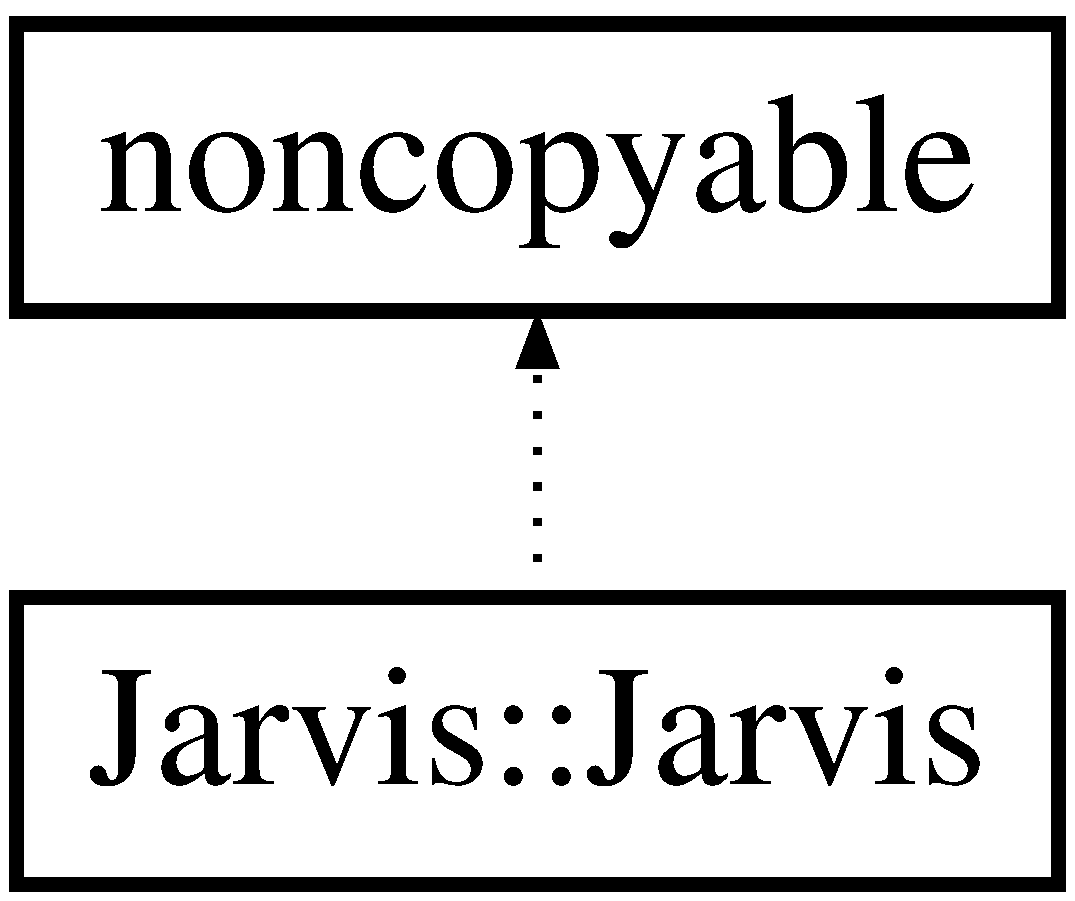
\includegraphics[height=2.000000cm]{classJarvis_1_1Jarvis}
\end{center}
\end{figure}
\subsection*{Открытые члены}
\begin{DoxyCompactItemize}
\item 
\mbox{\Hypertarget{classJarvis_1_1Jarvis_a34fb8baa346b1019769ea8b00c638dc4}\label{classJarvis_1_1Jarvis_a34fb8baa346b1019769ea8b00c638dc4}} 
\hyperlink{classJarvis_1_1Jarvis_a34fb8baa346b1019769ea8b00c638dc4}{Jarvis} ()=default
\begin{DoxyCompactList}\small\item\em Конструктор по-\/умолчанию \end{DoxyCompactList}\item 
\hyperlink{classJarvis_1_1Jarvis_ae6a7cc649ef8aabd836c8b549ab39507}{Jarvis} (\hyperlink{classJarvis_1_1Voice}{Voice} \&voice)
\begin{DoxyCompactList}\small\item\em Конструктор \end{DoxyCompactList}\item 
\mbox{\Hypertarget{classJarvis_1_1Jarvis_aa8670e3e8dfdd5e76cab8f57ccee5461}\label{classJarvis_1_1Jarvis_aa8670e3e8dfdd5e76cab8f57ccee5461}} 
\hyperlink{classJarvis_1_1Jarvis_aa8670e3e8dfdd5e76cab8f57ccee5461}{$\sim$\+Jarvis} ()=default
\begin{DoxyCompactList}\small\item\em Деструктор \end{DoxyCompactList}\item 
\mbox{\Hypertarget{classJarvis_1_1Jarvis_ac455d2a57de556bc9a8aa1b80fe99c99}\label{classJarvis_1_1Jarvis_ac455d2a57de556bc9a8aa1b80fe99c99}} 
{\bfseries Jarvis} (const \hyperlink{classJarvis_1_1Jarvis}{Jarvis} \&copy)=delete
\item 
\mbox{\Hypertarget{classJarvis_1_1Jarvis_abf77be09a8b7b116c31f26d17bd0851f}\label{classJarvis_1_1Jarvis_abf77be09a8b7b116c31f26d17bd0851f}} 
{\bfseries Jarvis} (\hyperlink{classJarvis_1_1Jarvis}{Jarvis} \&\&copy)=delete
\item 
\mbox{\Hypertarget{classJarvis_1_1Jarvis_a3488a3cc7ce01355c4537ba6dc517b65}\label{classJarvis_1_1Jarvis_a3488a3cc7ce01355c4537ba6dc517b65}} 
\hyperlink{classJarvis_1_1Jarvis}{Jarvis} \& {\bfseries operator=} (const \hyperlink{classJarvis_1_1Jarvis}{Jarvis} \&copy)=delete
\item 
\mbox{\Hypertarget{classJarvis_1_1Jarvis_aa6a5817a0c85b1a92e61aa5395f96d11}\label{classJarvis_1_1Jarvis_aa6a5817a0c85b1a92e61aa5395f96d11}} 
\hyperlink{classJarvis_1_1Jarvis}{Jarvis} \& {\bfseries operator=} (\hyperlink{classJarvis_1_1Jarvis}{Jarvis} \&\&copy)=delete
\item 
\mbox{\Hypertarget{classJarvis_1_1Jarvis_af74ffc81a286c827aed0ffc7efea1973}\label{classJarvis_1_1Jarvis_af74ffc81a286c827aed0ffc7efea1973}} 
\hyperlink{classJarvis_1_1Jarvis_af74ffc81a286c827aed0ffc7efea1973}{$\sim$\+Jarvis\+Destroyer} ()
\begin{DoxyCompactList}\small\item\em Деструктор \end{DoxyCompactList}\item 
void \hyperlink{classJarvis_1_1Jarvis_a1453f3e7f2587b7b884525c75d8b8cf5}{initialize} (\hyperlink{classJarvis_1_1Jarvis}{Jarvis} $\ast$jarvis)
\begin{DoxyCompactList}\small\item\em Инициализация системы \end{DoxyCompactList}\item 
\mbox{\Hypertarget{classJarvis_1_1Jarvis_a22a6798b7868c1f17ecf5023edbd252b}\label{classJarvis_1_1Jarvis_a22a6798b7868c1f17ecf5023edbd252b}} 
{\bfseries Jarvis\+Destroyer} (const Jarvis\+Destroyer \&copy)=delete
\item 
\mbox{\Hypertarget{classJarvis_1_1Jarvis_a382b3b739ed3881ae2d5a93b0743e72c}\label{classJarvis_1_1Jarvis_a382b3b739ed3881ae2d5a93b0743e72c}} 
{\bfseries Jarvis\+Destroyer} (Jarvis\+Destroyer \&\&copy)=delete
\item 
\mbox{\Hypertarget{classJarvis_1_1Jarvis_a449b426d29488b2004e8431dfeeb204b}\label{classJarvis_1_1Jarvis_a449b426d29488b2004e8431dfeeb204b}} 
Jarvis\+Destroyer \& {\bfseries operator=} (const Jarvis\+Destroyer \&copy)=delete
\item 
\mbox{\Hypertarget{classJarvis_1_1Jarvis_ace5b58fadb50698bbf9db3e0d7af3a2f}\label{classJarvis_1_1Jarvis_ace5b58fadb50698bbf9db3e0d7af3a2f}} 
Jarvis\+Destroyer \& {\bfseries operator=} (Jarvis\+Destroyer \&\&copy)=delete
\end{DoxyCompactItemize}
\subsection*{Открытые статические члены}
\begin{DoxyCompactItemize}
\item 
static \hyperlink{classJarvis_1_1Jarvis}{Jarvis} \& \hyperlink{classJarvis_1_1Jarvis_a6f50fbb249174da350352dc3429459b7}{instance} ()
\begin{DoxyCompactList}\small\item\em Инициализация системы \end{DoxyCompactList}\item 
static void \hyperlink{classJarvis_1_1Jarvis_a80c00115e07bf149673b3cf652751386}{say} (\hyperlink{classJarvis_1_1Voice}{Voice} \&voice, const say\+Phrase \&phrase)
\begin{DoxyCompactList}\small\item\em Воспроизведение фразы \end{DoxyCompactList}\item 
static string\+Voice \hyperlink{classJarvis_1_1Jarvis_a2a9f9ca691361b0ef640ac5a150acb39}{to\+Arduino} ()
\begin{DoxyCompactList}\small\item\em Статический метод для запуска скрипта \end{DoxyCompactList}\item 
static string\+Voice \hyperlink{classJarvis_1_1Jarvis_a4b45c41bc3fb910b2cf2f032b5fa0c08}{send\+To\+Yandex\+Speech\+Kit} ()
\begin{DoxyCompactList}\small\item\em Статический метод для \char`\"{}общения\char`\"{} с сервером Яндекса \end{DoxyCompactList}\item 
static void \hyperlink{classJarvis_1_1Jarvis_a211625e415e0aeb22eba6fab2deaa5e1}{send\+To\+Serial\+Port} (\hyperlink{classJarvis_1_1Arduino_1_1Connection_1_1SerialPort}{Serial\+Port} \&serial, const std\+::string \&command)
\begin{DoxyCompactList}\small\item\em Статический метод для \char`\"{}общения\char`\"{} с портом \hyperlink{namespaceArduino}{Arduino}. \end{DoxyCompactList}\item 
static map \hyperlink{classJarvis_1_1Jarvis_a5e7d9053e69eee8154c68e2bc86e7362}{get\+Map\+From\+Yandex\+Speech\+Kit} (const path\+To\+Configs \&path)
\begin{DoxyCompactList}\small\item\em Статический метод для \char`\"{}общения\char`\"{} получения данных с сервера Yandex. \end{DoxyCompactList}\end{DoxyCompactItemize}
\subsection*{Открытые атрибуты}
\begin{DoxyCompactItemize}
\item 
\mbox{\Hypertarget{classJarvis_1_1Jarvis_a8f581526d8e72ff7a086ea054008ad45}\label{classJarvis_1_1Jarvis_a8f581526d8e72ff7a086ea054008ad45}} 
private {\bfseries structs}\+: struct Jarvis\+Destroyer \+: boost\+::noncopyable \{ public methods\+: Jarvis\+Destroyer() = default
\item 
private \hyperlink{classJarvis_1_1Jarvis_a4009b6177d6dd3b01d550ba8d628b0ed}{params}\+: \hyperlink{classJarvis_1_1Jarvis}{Jarvis} $\ast$\+\_\+jarvis
\item 
\hyperlink{classJarvis_1_1Voice}{Voice} \hyperlink{classJarvis_1_1Jarvis_a52effab3870e7ba14e5a1fdbd5d2edc1}{\+\_\+voice}
\end{DoxyCompactItemize}
\subsection*{Статические открытые данные}
\begin{DoxyCompactItemize}
\item 
static Jarvis\+Destroyer \hyperlink{classJarvis_1_1Jarvis_ab2ccf0fd1be13af518d79c8c3adb2042}{\+\_\+destroyer}
\end{DoxyCompactItemize}
\subsection*{Друзья}
\begin{DoxyCompactItemize}
\item 
\mbox{\Hypertarget{classJarvis_1_1Jarvis_a2cc2b1b8510e686a8d6d42aeee07448d}\label{classJarvis_1_1Jarvis_a2cc2b1b8510e686a8d6d42aeee07448d}} 
struct {\bfseries Jarvis\+Destroyer}
\end{DoxyCompactItemize}


\subsection{Конструктор(ы)}
\mbox{\Hypertarget{classJarvis_1_1Jarvis_ae6a7cc649ef8aabd836c8b549ab39507}\label{classJarvis_1_1Jarvis_ae6a7cc649ef8aabd836c8b549ab39507}} 
\index{Jarvis\+::\+Jarvis@{Jarvis\+::\+Jarvis}!Jarvis@{Jarvis}}
\index{Jarvis@{Jarvis}!Jarvis\+::\+Jarvis@{Jarvis\+::\+Jarvis}}
\subsubsection{\texorpdfstring{Jarvis()}{Jarvis()}}
{\footnotesize\ttfamily Jarvis\+::\+Jarvis\+::\+Jarvis (\begin{DoxyParamCaption}\item[{\hyperlink{classJarvis_1_1Voice}{Voice} \&}]{voice }\end{DoxyParamCaption})}



Конструктор 


\begin{DoxyParams}{Аргументы}
{\em voice} & Голос \hyperlink{classJarvis_1_1Jarvis}{Jarvis}\textquotesingle{}a \\
\hline
\end{DoxyParams}


\subsection{Методы}
\mbox{\Hypertarget{classJarvis_1_1Jarvis_a5e7d9053e69eee8154c68e2bc86e7362}\label{classJarvis_1_1Jarvis_a5e7d9053e69eee8154c68e2bc86e7362}} 
\index{Jarvis\+::\+Jarvis@{Jarvis\+::\+Jarvis}!get\+Map\+From\+Yandex\+Speech\+Kit@{get\+Map\+From\+Yandex\+Speech\+Kit}}
\index{get\+Map\+From\+Yandex\+Speech\+Kit@{get\+Map\+From\+Yandex\+Speech\+Kit}!Jarvis\+::\+Jarvis@{Jarvis\+::\+Jarvis}}
\subsubsection{\texorpdfstring{get\+Map\+From\+Yandex\+Speech\+Kit()}{getMapFromYandexSpeechKit()}}
{\footnotesize\ttfamily static map Jarvis\+::\+Jarvis\+::get\+Map\+From\+Yandex\+Speech\+Kit (\begin{DoxyParamCaption}\item[{const path\+To\+Configs \&}]{path }\end{DoxyParamCaption})\hspace{0.3cm}{\ttfamily [static]}}



Статический метод для \char`\"{}общения\char`\"{} получения данных с сервера Yandex. 


\begin{DoxyParams}{Аргументы}
{\em path} & Путь до конфигурационного файла \\
\hline
\end{DoxyParams}
\begin{DoxyReturn}{Возвращает}
map Отображение вида std\+::string -\/$>$ std\+::string 
\end{DoxyReturn}
\mbox{\Hypertarget{classJarvis_1_1Jarvis_a1453f3e7f2587b7b884525c75d8b8cf5}\label{classJarvis_1_1Jarvis_a1453f3e7f2587b7b884525c75d8b8cf5}} 
\index{Jarvis\+::\+Jarvis@{Jarvis\+::\+Jarvis}!initialize@{initialize}}
\index{initialize@{initialize}!Jarvis\+::\+Jarvis@{Jarvis\+::\+Jarvis}}
\subsubsection{\texorpdfstring{initialize()}{initialize()}}
{\footnotesize\ttfamily void Jarvis\+::\+Jarvis\+::initialize (\begin{DoxyParamCaption}\item[{\hyperlink{classJarvis_1_1Jarvis}{Jarvis} $\ast$}]{jarvis }\end{DoxyParamCaption})}



Инициализация системы 


\begin{DoxyParams}{Аргументы}
{\em jarvis} & Объект \hyperlink{classJarvis_1_1Jarvis}{Jarvis} Метод для инициализации системы \\
\hline
\end{DoxyParams}
\mbox{\Hypertarget{classJarvis_1_1Jarvis_a6f50fbb249174da350352dc3429459b7}\label{classJarvis_1_1Jarvis_a6f50fbb249174da350352dc3429459b7}} 
\index{Jarvis\+::\+Jarvis@{Jarvis\+::\+Jarvis}!instance@{instance}}
\index{instance@{instance}!Jarvis\+::\+Jarvis@{Jarvis\+::\+Jarvis}}
\subsubsection{\texorpdfstring{instance()}{instance()}}
{\footnotesize\ttfamily static \hyperlink{classJarvis_1_1Jarvis}{Jarvis}\& Jarvis\+::\+Jarvis\+::instance (\begin{DoxyParamCaption}{ }\end{DoxyParamCaption})\hspace{0.3cm}{\ttfamily [static]}}



Инициализация системы 

\begin{DoxyReturn}{Возвращает}
\hyperlink{classJarvis_1_1Jarvis}{Jarvis} возвращает тип едиснтвенного объека \hyperlink{classJarvis_1_1Jarvis}{Jarvis} Метод для инициализации системы 
\end{DoxyReturn}
\mbox{\Hypertarget{classJarvis_1_1Jarvis_a80c00115e07bf149673b3cf652751386}\label{classJarvis_1_1Jarvis_a80c00115e07bf149673b3cf652751386}} 
\index{Jarvis\+::\+Jarvis@{Jarvis\+::\+Jarvis}!say@{say}}
\index{say@{say}!Jarvis\+::\+Jarvis@{Jarvis\+::\+Jarvis}}
\subsubsection{\texorpdfstring{say()}{say()}}
{\footnotesize\ttfamily static void Jarvis\+::\+Jarvis\+::say (\begin{DoxyParamCaption}\item[{\hyperlink{classJarvis_1_1Voice}{Voice} \&}]{voice,  }\item[{const say\+Phrase \&}]{phrase }\end{DoxyParamCaption})\hspace{0.3cm}{\ttfamily [static]}}



Воспроизведение фразы 


\begin{DoxyParams}{Аргументы}
{\em voice} & Голос \hyperlink{classJarvis_1_1Jarvis}{Jarvis} \\
\hline
{\em phrase} & Фраза, которую \hyperlink{classJarvis_1_1Jarvis}{Jarvis} должен вопроизвести голосом Метод для воспроизведения фразы, которую должен сказать \hyperlink{classJarvis_1_1Jarvis}{Jarvis} \\
\hline
\end{DoxyParams}
\mbox{\Hypertarget{classJarvis_1_1Jarvis_a211625e415e0aeb22eba6fab2deaa5e1}\label{classJarvis_1_1Jarvis_a211625e415e0aeb22eba6fab2deaa5e1}} 
\index{Jarvis\+::\+Jarvis@{Jarvis\+::\+Jarvis}!send\+To\+Serial\+Port@{send\+To\+Serial\+Port}}
\index{send\+To\+Serial\+Port@{send\+To\+Serial\+Port}!Jarvis\+::\+Jarvis@{Jarvis\+::\+Jarvis}}
\subsubsection{\texorpdfstring{send\+To\+Serial\+Port()}{sendToSerialPort()}}
{\footnotesize\ttfamily static void Jarvis\+::\+Jarvis\+::send\+To\+Serial\+Port (\begin{DoxyParamCaption}\item[{\hyperlink{classJarvis_1_1Arduino_1_1Connection_1_1SerialPort}{Serial\+Port} \&}]{serial,  }\item[{const std\+::string \&}]{command }\end{DoxyParamCaption})\hspace{0.3cm}{\ttfamily [static]}}



Статический метод для \char`\"{}общения\char`\"{} с портом \hyperlink{namespaceArduino}{Arduino}. 


\begin{DoxyParams}{Аргументы}
{\em serial} & Порт, по которому будет отправлен сигнал \\
\hline
{\em command} & Команда, которая будет отправлена \\
\hline
\end{DoxyParams}
\mbox{\Hypertarget{classJarvis_1_1Jarvis_a4b45c41bc3fb910b2cf2f032b5fa0c08}\label{classJarvis_1_1Jarvis_a4b45c41bc3fb910b2cf2f032b5fa0c08}} 
\index{Jarvis\+::\+Jarvis@{Jarvis\+::\+Jarvis}!send\+To\+Yandex\+Speech\+Kit@{send\+To\+Yandex\+Speech\+Kit}}
\index{send\+To\+Yandex\+Speech\+Kit@{send\+To\+Yandex\+Speech\+Kit}!Jarvis\+::\+Jarvis@{Jarvis\+::\+Jarvis}}
\subsubsection{\texorpdfstring{send\+To\+Yandex\+Speech\+Kit()}{sendToYandexSpeechKit()}}
{\footnotesize\ttfamily static string\+Voice Jarvis\+::\+Jarvis\+::send\+To\+Yandex\+Speech\+Kit (\begin{DoxyParamCaption}{ }\end{DoxyParamCaption})\hspace{0.3cm}{\ttfamily [static]}}



Статический метод для \char`\"{}общения\char`\"{} с сервером Яндекса 

\begin{DoxyReturn}{Возвращает}
string\+Voice Строка, преобразованная из голоса 
\end{DoxyReturn}
\mbox{\Hypertarget{classJarvis_1_1Jarvis_a2a9f9ca691361b0ef640ac5a150acb39}\label{classJarvis_1_1Jarvis_a2a9f9ca691361b0ef640ac5a150acb39}} 
\index{Jarvis\+::\+Jarvis@{Jarvis\+::\+Jarvis}!to\+Arduino@{to\+Arduino}}
\index{to\+Arduino@{to\+Arduino}!Jarvis\+::\+Jarvis@{Jarvis\+::\+Jarvis}}
\subsubsection{\texorpdfstring{to\+Arduino()}{toArduino()}}
{\footnotesize\ttfamily static string\+Voice Jarvis\+::\+Jarvis\+::to\+Arduino (\begin{DoxyParamCaption}{ }\end{DoxyParamCaption})\hspace{0.3cm}{\ttfamily [static]}}



Статический метод для запуска скрипта 

\begin{DoxyReturn}{Возвращает}
string\+Voice Строка, преобразованная из голоса 
\end{DoxyReturn}


\subsection{Данные класса}
\mbox{\Hypertarget{classJarvis_1_1Jarvis_ab2ccf0fd1be13af518d79c8c3adb2042}\label{classJarvis_1_1Jarvis_ab2ccf0fd1be13af518d79c8c3adb2042}} 
\index{Jarvis\+::\+Jarvis@{Jarvis\+::\+Jarvis}!\+\_\+destroyer@{\+\_\+destroyer}}
\index{\+\_\+destroyer@{\+\_\+destroyer}!Jarvis\+::\+Jarvis@{Jarvis\+::\+Jarvis}}
\subsubsection{\texorpdfstring{\+\_\+destroyer}{\_destroyer}}
{\footnotesize\ttfamily Jarvis\+Destroyer Jarvis\+::\+Jarvis\+::\+\_\+destroyer\hspace{0.3cm}{\ttfamily [static]}}

Статический объект, отвечающий за разрушение \hyperlink{classJarvis_1_1Jarvis}{Jarvis}\textquotesingle{}a \mbox{\Hypertarget{classJarvis_1_1Jarvis_a52effab3870e7ba14e5a1fdbd5d2edc1}\label{classJarvis_1_1Jarvis_a52effab3870e7ba14e5a1fdbd5d2edc1}} 
\index{Jarvis\+::\+Jarvis@{Jarvis\+::\+Jarvis}!\+\_\+voice@{\+\_\+voice}}
\index{\+\_\+voice@{\+\_\+voice}!Jarvis\+::\+Jarvis@{Jarvis\+::\+Jarvis}}
\subsubsection{\texorpdfstring{\+\_\+voice}{\_voice}}
{\footnotesize\ttfamily \hyperlink{classJarvis_1_1Voice}{Voice} Jarvis\+::\+Jarvis\+::\+\_\+voice}

Голос \hyperlink{classJarvis_1_1Jarvis}{Jarvis} \mbox{\Hypertarget{classJarvis_1_1Jarvis_a4009b6177d6dd3b01d550ba8d628b0ed}\label{classJarvis_1_1Jarvis_a4009b6177d6dd3b01d550ba8d628b0ed}} 
\index{Jarvis\+::\+Jarvis@{Jarvis\+::\+Jarvis}!params@{params}}
\index{params@{params}!Jarvis\+::\+Jarvis@{Jarvis\+::\+Jarvis}}
\subsubsection{\texorpdfstring{params}{params}}
{\footnotesize\ttfamily private Jarvis\+::\+Jarvis\+::params}

Объект \hyperlink{classJarvis_1_1Jarvis}{Jarvis}

Статический объект \hyperlink{classJarvis_1_1Jarvis}{Jarvis} 

Объявления и описания членов класса находятся в файле\+:\begin{DoxyCompactItemize}
\item 
/\+Users/vladislavpereskokov/\+Desktop/\+Jarvis/\+Voice/include/Jarvis.\+hpp\end{DoxyCompactItemize}

\hypertarget{classJarvis}{}\section{Класс Jarvis}
\label{classJarvis}\index{Jarvis@{Jarvis}}


Класс, описывающий аналог ИИ  




{\ttfamily \#include $<$Jarvis.\+hpp$>$}



\subsection{Подробное описание}
Класс, описывающий аналог ИИ 

Объявления и описания членов класса находятся в файле\+:\begin{DoxyCompactItemize}
\item 
/\+Users/vladislavpereskokov/\+Desktop/\+Jarvis/\+Voice/include/Jarvis.\+hpp\end{DoxyCompactItemize}

\hypertarget{classJarvis_1_1Parser}{}\section{Класс Jarvis\+:\+:Parser}
\label{classJarvis_1_1Parser}\index{Jarvis\+::\+Parser@{Jarvis\+::\+Parser}}


Класс для парсинга файлов различных типов  




{\ttfamily \#include $<$Parser.\+hpp$>$}

\subsection*{Открытые члены}
\begin{DoxyCompactItemize}
\item 
\mbox{\Hypertarget{classJarvis_1_1Parser_a60c7c20f5314859c9f204dd5142fcf90}\label{classJarvis_1_1Parser_a60c7c20f5314859c9f204dd5142fcf90}} 
\hyperlink{classJarvis_1_1Parser_a60c7c20f5314859c9f204dd5142fcf90}{Parser} ()=default
\begin{DoxyCompactList}\small\item\em Конструктор по-\/умолчанию \end{DoxyCompactList}\item 
\hyperlink{classJarvis_1_1Parser_ac4987517b9f2618f1c8a7ff8a91f6b77}{Parser} (const Path \&path)
\begin{DoxyCompactList}\small\item\em Конструктор \end{DoxyCompactList}\item 
\mbox{\Hypertarget{classJarvis_1_1Parser_a42970c65127a01194e31175af54cd292}\label{classJarvis_1_1Parser_a42970c65127a01194e31175af54cd292}} 
\hyperlink{classJarvis_1_1Parser_a42970c65127a01194e31175af54cd292}{Parser} (const \hyperlink{classJarvis_1_1Parser}{Parser} \&copy)=default
\begin{DoxyCompactList}\small\item\em Конструктор копирования \end{DoxyCompactList}\item 
\mbox{\Hypertarget{classJarvis_1_1Parser_a4cc69248743fb4bcaa27ebe8ca60d4bf}\label{classJarvis_1_1Parser_a4cc69248743fb4bcaa27ebe8ca60d4bf}} 
\hyperlink{classJarvis_1_1Parser}{Parser} \& \hyperlink{classJarvis_1_1Parser_a4cc69248743fb4bcaa27ebe8ca60d4bf}{operator=} (const \hyperlink{classJarvis_1_1Parser}{Parser} \&copy)=default
\begin{DoxyCompactList}\small\item\em Оператор копирования \end{DoxyCompactList}\item 
\mbox{\Hypertarget{classJarvis_1_1Parser_a7ff8a13f47d05e0fe46ce9b90cf596fd}\label{classJarvis_1_1Parser_a7ff8a13f47d05e0fe46ce9b90cf596fd}} 
\hyperlink{classJarvis_1_1Parser_a7ff8a13f47d05e0fe46ce9b90cf596fd}{$\sim$\+Parser} ()=default
\begin{DoxyCompactList}\small\item\em Деструктор \end{DoxyCompactList}\item 
void \hyperlink{classJarvis_1_1Parser_ae2e8ce2a61c865342619fffe478dcda3}{load\+Target} (const Path \&path)
\begin{DoxyCompactList}\small\item\em Метод для подгрузки файла \end{DoxyCompactList}\item 
Tree \hyperlink{classJarvis_1_1Parser_a6d9a642092d5b7806b19ea6ccd98a515}{json\+Parse} ()
\begin{DoxyCompactList}\small\item\em Парсер json фалйа \end{DoxyCompactList}\item 
Tree \hyperlink{classJarvis_1_1Parser_ae970d807833a09eb01ac2bb3367560b7}{xml\+Parse} ()
\begin{DoxyCompactList}\small\item\em Парсер xml фалйа \end{DoxyCompactList}\end{DoxyCompactItemize}
\subsection*{Открытые атрибуты}
\begin{DoxyCompactItemize}
\item 
private \hyperlink{classJarvis_1_1Parser_a60503f54d37de6bc5eac1e6cb0c79c88}{params}\+: Path \+\_\+target
\item 
Tree \hyperlink{classJarvis_1_1Parser_aaa45f2682e516630116ab3a80028d0d4}{\+\_\+tree}
\end{DoxyCompactItemize}
\subsection*{Друзья}
\begin{DoxyCompactItemize}
\item 
Tree \hyperlink{classJarvis_1_1Parser_ac52ba088bbd034ec108efce6c8f48e17}{json\+Parse} (string\+Target \&stream)
\begin{DoxyCompactList}\small\item\em Парсер json фалйа \end{DoxyCompactList}\item 
Tree \hyperlink{classJarvis_1_1Parser_a6f226036ccce1dd03cab22a3214374f4}{xml\+Parse} (string\+Target \&stream)
\begin{DoxyCompactList}\small\item\em Парсер xml фалйа \end{DoxyCompactList}\end{DoxyCompactItemize}


\subsection{Подробное описание}
Класс для парсинга файлов различных типов 

\subsection{Конструктор(ы)}
\mbox{\Hypertarget{classJarvis_1_1Parser_ac4987517b9f2618f1c8a7ff8a91f6b77}\label{classJarvis_1_1Parser_ac4987517b9f2618f1c8a7ff8a91f6b77}} 
\index{Jarvis\+::\+Parser@{Jarvis\+::\+Parser}!Parser@{Parser}}
\index{Parser@{Parser}!Jarvis\+::\+Parser@{Jarvis\+::\+Parser}}
\subsubsection{\texorpdfstring{Parser()}{Parser()}}
{\footnotesize\ttfamily Jarvis\+::\+Parser\+::\+Parser (\begin{DoxyParamCaption}\item[{const Path \&}]{path }\end{DoxyParamCaption})\hspace{0.3cm}{\ttfamily [explicit]}}



Конструктор 


\begin{DoxyParams}{Аргументы}
{\em path} & Путь до файла \\
\hline
\end{DoxyParams}


\subsection{Методы}
\mbox{\Hypertarget{classJarvis_1_1Parser_a6d9a642092d5b7806b19ea6ccd98a515}\label{classJarvis_1_1Parser_a6d9a642092d5b7806b19ea6ccd98a515}} 
\index{Jarvis\+::\+Parser@{Jarvis\+::\+Parser}!json\+Parse@{json\+Parse}}
\index{json\+Parse@{json\+Parse}!Jarvis\+::\+Parser@{Jarvis\+::\+Parser}}
\subsubsection{\texorpdfstring{json\+Parse()}{jsonParse()}}
{\footnotesize\ttfamily Tree Jarvis\+::\+Parser\+::json\+Parse (\begin{DoxyParamCaption}{ }\end{DoxyParamCaption})}



Парсер json фалйа 

\begin{DoxyReturn}{Возвращает}
Дерево, распарсенного файла 
\end{DoxyReturn}
\mbox{\Hypertarget{classJarvis_1_1Parser_ae2e8ce2a61c865342619fffe478dcda3}\label{classJarvis_1_1Parser_ae2e8ce2a61c865342619fffe478dcda3}} 
\index{Jarvis\+::\+Parser@{Jarvis\+::\+Parser}!load\+Target@{load\+Target}}
\index{load\+Target@{load\+Target}!Jarvis\+::\+Parser@{Jarvis\+::\+Parser}}
\subsubsection{\texorpdfstring{load\+Target()}{loadTarget()}}
{\footnotesize\ttfamily void Jarvis\+::\+Parser\+::load\+Target (\begin{DoxyParamCaption}\item[{const Path \&}]{path }\end{DoxyParamCaption})}



Метод для подгрузки файла 


\begin{DoxyParams}{Аргументы}
{\em path} & Путь до файла \\
\hline
\end{DoxyParams}
\mbox{\Hypertarget{classJarvis_1_1Parser_ae970d807833a09eb01ac2bb3367560b7}\label{classJarvis_1_1Parser_ae970d807833a09eb01ac2bb3367560b7}} 
\index{Jarvis\+::\+Parser@{Jarvis\+::\+Parser}!xml\+Parse@{xml\+Parse}}
\index{xml\+Parse@{xml\+Parse}!Jarvis\+::\+Parser@{Jarvis\+::\+Parser}}
\subsubsection{\texorpdfstring{xml\+Parse()}{xmlParse()}}
{\footnotesize\ttfamily Tree Jarvis\+::\+Parser\+::xml\+Parse (\begin{DoxyParamCaption}{ }\end{DoxyParamCaption})}



Парсер xml фалйа 

\begin{DoxyReturn}{Возвращает}
Дерево, распарсенного файла 
\end{DoxyReturn}


\subsection{Документация по друзьям класса и функциям, относящимся к классу}
\mbox{\Hypertarget{classJarvis_1_1Parser_ac52ba088bbd034ec108efce6c8f48e17}\label{classJarvis_1_1Parser_ac52ba088bbd034ec108efce6c8f48e17}} 
\index{Jarvis\+::\+Parser@{Jarvis\+::\+Parser}!json\+Parse@{json\+Parse}}
\index{json\+Parse@{json\+Parse}!Jarvis\+::\+Parser@{Jarvis\+::\+Parser}}
\subsubsection{\texorpdfstring{json\+Parse}{jsonParse}}
{\footnotesize\ttfamily Tree json\+Parse (\begin{DoxyParamCaption}\item[{Parser\+::string\+Target \&}]{stream }\end{DoxyParamCaption})\hspace{0.3cm}{\ttfamily [friend]}}



Парсер json фалйа 

\begin{DoxyReturn}{Возвращает}
Дерево, распарсенного файла 
\end{DoxyReturn}
\mbox{\Hypertarget{classJarvis_1_1Parser_a6f226036ccce1dd03cab22a3214374f4}\label{classJarvis_1_1Parser_a6f226036ccce1dd03cab22a3214374f4}} 
\index{Jarvis\+::\+Parser@{Jarvis\+::\+Parser}!xml\+Parse@{xml\+Parse}}
\index{xml\+Parse@{xml\+Parse}!Jarvis\+::\+Parser@{Jarvis\+::\+Parser}}
\subsubsection{\texorpdfstring{xml\+Parse}{xmlParse}}
{\footnotesize\ttfamily Tree xml\+Parse (\begin{DoxyParamCaption}\item[{Parser\+::string\+Target \&}]{stream }\end{DoxyParamCaption})\hspace{0.3cm}{\ttfamily [friend]}}



Парсер xml фалйа 

\begin{DoxyReturn}{Возвращает}
Дерево, распарсенного файла 
\end{DoxyReturn}


\subsection{Данные класса}
\mbox{\Hypertarget{classJarvis_1_1Parser_aaa45f2682e516630116ab3a80028d0d4}\label{classJarvis_1_1Parser_aaa45f2682e516630116ab3a80028d0d4}} 
\index{Jarvis\+::\+Parser@{Jarvis\+::\+Parser}!\+\_\+tree@{\+\_\+tree}}
\index{\+\_\+tree@{\+\_\+tree}!Jarvis\+::\+Parser@{Jarvis\+::\+Parser}}
\subsubsection{\texorpdfstring{\+\_\+tree}{\_tree}}
{\footnotesize\ttfamily Tree Jarvis\+::\+Parser\+::\+\_\+tree}

Дерево \mbox{\Hypertarget{classJarvis_1_1Parser_a60503f54d37de6bc5eac1e6cb0c79c88}\label{classJarvis_1_1Parser_a60503f54d37de6bc5eac1e6cb0c79c88}} 
\index{Jarvis\+::\+Parser@{Jarvis\+::\+Parser}!params@{params}}
\index{params@{params}!Jarvis\+::\+Parser@{Jarvis\+::\+Parser}}
\subsubsection{\texorpdfstring{params}{params}}
{\footnotesize\ttfamily private Jarvis\+::\+Parser\+::params}

путь до файла 

Объявления и описания членов класса находятся в файле\+:\begin{DoxyCompactItemize}
\item 
/\+Users/vladislavpereskokov/\+Desktop/\+Jarvis/\+Voice/include/Parser.\+hpp\end{DoxyCompactItemize}

\hypertarget{classJarvis_1_1Sentence}{}\section{Класс Jarvis\+:\+:Sentence}
\label{classJarvis_1_1Sentence}\index{Jarvis\+::\+Sentence@{Jarvis\+::\+Sentence}}


Класс для работы с предложениями к \hyperlink{classJarvis_1_1Jarvis}{Jarvis}.  




{\ttfamily \#include $<$Sentence.\+hpp$>$}

\subsection*{Открытые члены}
\begin{DoxyCompactItemize}
\item 
\hyperlink{classJarvis_1_1Sentence_acc720056eaf5ae72302802c6ef694fcd}{Sentence} (const phrase \&phrase)
\begin{DoxyCompactList}\small\item\em Конструктор \end{DoxyCompactList}\item 
\hyperlink{classJarvis_1_1Sentence_a2cf95d90b62afeb1ba141157220b469d}{Sentence} (const \hyperlink{classJarvis_1_1Sentence}{Sentence} \&copy)
\begin{DoxyCompactList}\small\item\em Конструктор копирования \end{DoxyCompactList}\item 
\hyperlink{classJarvis_1_1Sentence_af852c6a73ee0411f4c0f78ed68f97bd3}{Sentence} (\hyperlink{classJarvis_1_1Sentence}{Sentence} \&\&copy)
\begin{DoxyCompactList}\small\item\em Конструктор копирования \end{DoxyCompactList}\item 
\hyperlink{classJarvis_1_1Sentence}{Sentence} \& \hyperlink{classJarvis_1_1Sentence_a023e7f01ec0e27b0451206c1be002fda}{operator=} (const \hyperlink{classJarvis_1_1Sentence}{Sentence} \&copy)
\begin{DoxyCompactList}\small\item\em Оператор копирования \end{DoxyCompactList}\item 
\hyperlink{classJarvis_1_1Sentence}{Sentence} \& \hyperlink{classJarvis_1_1Sentence_a5f9db983639fc70219bf1a55033fe5ed}{operator=} (\hyperlink{classJarvis_1_1Sentence}{Sentence} \&\&copy)
\begin{DoxyCompactList}\small\item\em Оператор копирования \end{DoxyCompactList}\item 
\mbox{\Hypertarget{classJarvis_1_1Sentence_ae75a8146136428d9089f3698a857276f}\label{classJarvis_1_1Sentence_ae75a8146136428d9089f3698a857276f}} 
\hyperlink{classJarvis_1_1Sentence_ae75a8146136428d9089f3698a857276f}{$\sim$\+Sentence} ()=default
\begin{DoxyCompactList}\small\item\em Деструктор \end{DoxyCompactList}\item 
void \hyperlink{classJarvis_1_1Sentence_a9663bb38ce80ea245bc8fb33e04fc41f}{set\+Sentence} (const \hyperlink{classJarvis_1_1Sentence}{Sentence} \&sentence)
\begin{DoxyCompactList}\small\item\em Метод добавления фразы \end{DoxyCompactList}\item 
void \hyperlink{classJarvis_1_1Sentence_ad026c842e31491b85f2f6f186667c799}{set\+Sentence} (const phrase \&phrase)
\begin{DoxyCompactList}\small\item\em Метод добавления фразы \end{DoxyCompactList}\item 
phrase \hyperlink{classJarvis_1_1Sentence_a480b97ff340eba0a4dcb505aefa26d40}{get\+Sentence} () const
\begin{DoxyCompactList}\small\item\em Метод добавления фразы \end{DoxyCompactList}\end{DoxyCompactItemize}
\subsection*{Открытые атрибуты}
\begin{DoxyCompactItemize}
\item 
private \hyperlink{classJarvis_1_1Sentence_a9a5cdde8bf7dc872ec20ff6afac01a0a}{params}\+: phrase \+\_\+phrase
\end{DoxyCompactItemize}
\subsection*{Друзья}
\begin{DoxyCompactItemize}
\item 
bool \hyperlink{classJarvis_1_1Sentence_a6ecb6a1aa4a36b15b8871048ec240467}{operator==} (const \hyperlink{classJarvis_1_1Sentence}{Sentence} \&lhs, const \hyperlink{classJarvis_1_1Sentence}{Sentence} \&rhs)
\begin{DoxyCompactList}\small\item\em Оператор сравнения \end{DoxyCompactList}\item 
bool \hyperlink{classJarvis_1_1Sentence_ab281eae311e630f9dca86a48fc608518}{operator!=} (const \hyperlink{classJarvis_1_1Sentence}{Sentence} \&lhs, const \hyperlink{classJarvis_1_1Sentence}{Sentence} \&rhs)
\begin{DoxyCompactList}\small\item\em Оператор сравнения \end{DoxyCompactList}\item 
bool \hyperlink{classJarvis_1_1Sentence_a90cda2640b9dadd4b19c9baae07fe55d}{operator$>$} (const \hyperlink{classJarvis_1_1Sentence}{Sentence} \&lhs, const \hyperlink{classJarvis_1_1Sentence}{Sentence} \&rhs)
\begin{DoxyCompactList}\small\item\em Оператор больше \end{DoxyCompactList}\item 
bool \hyperlink{classJarvis_1_1Sentence_ad8bc9f0888e1331f783f7a8e1765403f}{operator$<$} (const \hyperlink{classJarvis_1_1Sentence}{Sentence} \&lhs, const \hyperlink{classJarvis_1_1Sentence}{Sentence} \&rhs)
\begin{DoxyCompactList}\small\item\em Оператор меньше \end{DoxyCompactList}\item 
bool \hyperlink{classJarvis_1_1Sentence_a4e0a564a452ba4172bd0d718c04ea7e0}{operator$>$=} (const \hyperlink{classJarvis_1_1Sentence}{Sentence} \&lhs, const \hyperlink{classJarvis_1_1Sentence}{Sentence} \&rhs)
\begin{DoxyCompactList}\small\item\em Оператор больше или равно \end{DoxyCompactList}\item 
bool \hyperlink{classJarvis_1_1Sentence_af9d0c048412448422e8af2e420a0be48}{operator$<$=} (const \hyperlink{classJarvis_1_1Sentence}{Sentence} \&lhs, const \hyperlink{classJarvis_1_1Sentence}{Sentence} \&rhs)
\begin{DoxyCompactList}\small\item\em Оператор меньше или равно \end{DoxyCompactList}\end{DoxyCompactItemize}


\subsection{Подробное описание}
Класс для работы с предложениями к \hyperlink{classJarvis_1_1Jarvis}{Jarvis}. 

\subsection{Конструктор(ы)}
\mbox{\Hypertarget{classJarvis_1_1Sentence_acc720056eaf5ae72302802c6ef694fcd}\label{classJarvis_1_1Sentence_acc720056eaf5ae72302802c6ef694fcd}} 
\index{Jarvis\+::\+Sentence@{Jarvis\+::\+Sentence}!Sentence@{Sentence}}
\index{Sentence@{Sentence}!Jarvis\+::\+Sentence@{Jarvis\+::\+Sentence}}
\subsubsection{\texorpdfstring{Sentence()}{Sentence()}\hspace{0.1cm}{\footnotesize\ttfamily [1/3]}}
{\footnotesize\ttfamily Jarvis\+::\+Sentence\+::\+Sentence (\begin{DoxyParamCaption}\item[{const phrase \&}]{phrase }\end{DoxyParamCaption})}



Конструктор 


\begin{DoxyParams}{Аргументы}
{\em phrase} & Фраза \\
\hline
\end{DoxyParams}
\mbox{\Hypertarget{classJarvis_1_1Sentence_a2cf95d90b62afeb1ba141157220b469d}\label{classJarvis_1_1Sentence_a2cf95d90b62afeb1ba141157220b469d}} 
\index{Jarvis\+::\+Sentence@{Jarvis\+::\+Sentence}!Sentence@{Sentence}}
\index{Sentence@{Sentence}!Jarvis\+::\+Sentence@{Jarvis\+::\+Sentence}}
\subsubsection{\texorpdfstring{Sentence()}{Sentence()}\hspace{0.1cm}{\footnotesize\ttfamily [2/3]}}
{\footnotesize\ttfamily Jarvis\+::\+Sentence\+::\+Sentence (\begin{DoxyParamCaption}\item[{const \hyperlink{classJarvis_1_1Sentence}{Sentence} \&}]{copy }\end{DoxyParamCaption})}



Конструктор копирования 


\begin{DoxyParams}{Аргументы}
{\em copy} & Копируемый объект \\
\hline
\end{DoxyParams}
\mbox{\Hypertarget{classJarvis_1_1Sentence_af852c6a73ee0411f4c0f78ed68f97bd3}\label{classJarvis_1_1Sentence_af852c6a73ee0411f4c0f78ed68f97bd3}} 
\index{Jarvis\+::\+Sentence@{Jarvis\+::\+Sentence}!Sentence@{Sentence}}
\index{Sentence@{Sentence}!Jarvis\+::\+Sentence@{Jarvis\+::\+Sentence}}
\subsubsection{\texorpdfstring{Sentence()}{Sentence()}\hspace{0.1cm}{\footnotesize\ttfamily [3/3]}}
{\footnotesize\ttfamily Jarvis\+::\+Sentence\+::\+Sentence (\begin{DoxyParamCaption}\item[{\hyperlink{classJarvis_1_1Sentence}{Sentence} \&\&}]{copy }\end{DoxyParamCaption})}



Конструктор копирования 


\begin{DoxyParams}{Аргументы}
{\em copy} & Копируемый объект \\
\hline
\end{DoxyParams}


\subsection{Методы}
\mbox{\Hypertarget{classJarvis_1_1Sentence_a480b97ff340eba0a4dcb505aefa26d40}\label{classJarvis_1_1Sentence_a480b97ff340eba0a4dcb505aefa26d40}} 
\index{Jarvis\+::\+Sentence@{Jarvis\+::\+Sentence}!get\+Sentence@{get\+Sentence}}
\index{get\+Sentence@{get\+Sentence}!Jarvis\+::\+Sentence@{Jarvis\+::\+Sentence}}
\subsubsection{\texorpdfstring{get\+Sentence()}{getSentence()}}
{\footnotesize\ttfamily phrase Jarvis\+::\+Sentence\+::get\+Sentence (\begin{DoxyParamCaption}{ }\end{DoxyParamCaption}) const}



Метод добавления фразы 

\begin{DoxyReturn}{Возвращает}
Фраза (строка) 
\end{DoxyReturn}
\mbox{\Hypertarget{classJarvis_1_1Sentence_a023e7f01ec0e27b0451206c1be002fda}\label{classJarvis_1_1Sentence_a023e7f01ec0e27b0451206c1be002fda}} 
\index{Jarvis\+::\+Sentence@{Jarvis\+::\+Sentence}!operator=@{operator=}}
\index{operator=@{operator=}!Jarvis\+::\+Sentence@{Jarvis\+::\+Sentence}}
\subsubsection{\texorpdfstring{operator=()}{operator=()}\hspace{0.1cm}{\footnotesize\ttfamily [1/2]}}
{\footnotesize\ttfamily \hyperlink{classJarvis_1_1Sentence}{Sentence}\& Jarvis\+::\+Sentence\+::operator= (\begin{DoxyParamCaption}\item[{const \hyperlink{classJarvis_1_1Sentence}{Sentence} \&}]{copy }\end{DoxyParamCaption})}



Оператор копирования 


\begin{DoxyParams}{Аргументы}
{\em copy} & Копируемый объект \\
\hline
\end{DoxyParams}
\mbox{\Hypertarget{classJarvis_1_1Sentence_a5f9db983639fc70219bf1a55033fe5ed}\label{classJarvis_1_1Sentence_a5f9db983639fc70219bf1a55033fe5ed}} 
\index{Jarvis\+::\+Sentence@{Jarvis\+::\+Sentence}!operator=@{operator=}}
\index{operator=@{operator=}!Jarvis\+::\+Sentence@{Jarvis\+::\+Sentence}}
\subsubsection{\texorpdfstring{operator=()}{operator=()}\hspace{0.1cm}{\footnotesize\ttfamily [2/2]}}
{\footnotesize\ttfamily \hyperlink{classJarvis_1_1Sentence}{Sentence}\& Jarvis\+::\+Sentence\+::operator= (\begin{DoxyParamCaption}\item[{\hyperlink{classJarvis_1_1Sentence}{Sentence} \&\&}]{copy }\end{DoxyParamCaption})}



Оператор копирования 


\begin{DoxyParams}{Аргументы}
{\em copy} & Копируемый объект \\
\hline
\end{DoxyParams}
\mbox{\Hypertarget{classJarvis_1_1Sentence_a9663bb38ce80ea245bc8fb33e04fc41f}\label{classJarvis_1_1Sentence_a9663bb38ce80ea245bc8fb33e04fc41f}} 
\index{Jarvis\+::\+Sentence@{Jarvis\+::\+Sentence}!set\+Sentence@{set\+Sentence}}
\index{set\+Sentence@{set\+Sentence}!Jarvis\+::\+Sentence@{Jarvis\+::\+Sentence}}
\subsubsection{\texorpdfstring{set\+Sentence()}{setSentence()}\hspace{0.1cm}{\footnotesize\ttfamily [1/2]}}
{\footnotesize\ttfamily void Jarvis\+::\+Sentence\+::set\+Sentence (\begin{DoxyParamCaption}\item[{const \hyperlink{classJarvis_1_1Sentence}{Sentence} \&}]{sentence }\end{DoxyParamCaption})}



Метод добавления фразы 


\begin{DoxyParams}{Аргументы}
{\em sentence} & Фраза \\
\hline
\end{DoxyParams}
\mbox{\Hypertarget{classJarvis_1_1Sentence_ad026c842e31491b85f2f6f186667c799}\label{classJarvis_1_1Sentence_ad026c842e31491b85f2f6f186667c799}} 
\index{Jarvis\+::\+Sentence@{Jarvis\+::\+Sentence}!set\+Sentence@{set\+Sentence}}
\index{set\+Sentence@{set\+Sentence}!Jarvis\+::\+Sentence@{Jarvis\+::\+Sentence}}
\subsubsection{\texorpdfstring{set\+Sentence()}{setSentence()}\hspace{0.1cm}{\footnotesize\ttfamily [2/2]}}
{\footnotesize\ttfamily void Jarvis\+::\+Sentence\+::set\+Sentence (\begin{DoxyParamCaption}\item[{const phrase \&}]{phrase }\end{DoxyParamCaption})}



Метод добавления фразы 


\begin{DoxyParams}{Аргументы}
{\em phrase} & Фраза (строка) \\
\hline
\end{DoxyParams}


\subsection{Документация по друзьям класса и функциям, относящимся к классу}
\mbox{\Hypertarget{classJarvis_1_1Sentence_ab281eae311e630f9dca86a48fc608518}\label{classJarvis_1_1Sentence_ab281eae311e630f9dca86a48fc608518}} 
\index{Jarvis\+::\+Sentence@{Jarvis\+::\+Sentence}!operator"!=@{operator"!=}}
\index{operator"!=@{operator"!=}!Jarvis\+::\+Sentence@{Jarvis\+::\+Sentence}}
\subsubsection{\texorpdfstring{operator"!=}{operator!=}}
{\footnotesize\ttfamily bool operator!= (\begin{DoxyParamCaption}\item[{const \hyperlink{classJarvis_1_1Sentence}{Sentence} \&}]{lhs,  }\item[{const \hyperlink{classJarvis_1_1Sentence}{Sentence} \&}]{rhs }\end{DoxyParamCaption})\hspace{0.3cm}{\ttfamily [friend]}}



Оператор сравнения 


\begin{DoxyParams}{Аргументы}
{\em lhs} & Левый операнд \\
\hline
{\em rhs} & Правый операнд \\
\hline
\end{DoxyParams}
\begin{DoxyReturn}{Возвращает}
bool Результат сравнения 
\end{DoxyReturn}
\mbox{\Hypertarget{classJarvis_1_1Sentence_ad8bc9f0888e1331f783f7a8e1765403f}\label{classJarvis_1_1Sentence_ad8bc9f0888e1331f783f7a8e1765403f}} 
\index{Jarvis\+::\+Sentence@{Jarvis\+::\+Sentence}!operator$<$@{operator$<$}}
\index{operator$<$@{operator$<$}!Jarvis\+::\+Sentence@{Jarvis\+::\+Sentence}}
\subsubsection{\texorpdfstring{operator$<$}{operator<}}
{\footnotesize\ttfamily bool operator$<$ (\begin{DoxyParamCaption}\item[{const \hyperlink{classJarvis_1_1Sentence}{Sentence} \&}]{lhs,  }\item[{const \hyperlink{classJarvis_1_1Sentence}{Sentence} \&}]{rhs }\end{DoxyParamCaption})\hspace{0.3cm}{\ttfamily [friend]}}



Оператор меньше 


\begin{DoxyParams}{Аргументы}
{\em lhs} & Левый операнд \\
\hline
{\em rhs} & Правый операнд \\
\hline
\end{DoxyParams}
\begin{DoxyReturn}{Возвращает}
bool Результат сравнения 
\end{DoxyReturn}
\mbox{\Hypertarget{classJarvis_1_1Sentence_af9d0c048412448422e8af2e420a0be48}\label{classJarvis_1_1Sentence_af9d0c048412448422e8af2e420a0be48}} 
\index{Jarvis\+::\+Sentence@{Jarvis\+::\+Sentence}!operator$<$=@{operator$<$=}}
\index{operator$<$=@{operator$<$=}!Jarvis\+::\+Sentence@{Jarvis\+::\+Sentence}}
\subsubsection{\texorpdfstring{operator$<$=}{operator<=}}
{\footnotesize\ttfamily bool operator$<$= (\begin{DoxyParamCaption}\item[{const \hyperlink{classJarvis_1_1Sentence}{Sentence} \&}]{lhs,  }\item[{const \hyperlink{classJarvis_1_1Sentence}{Sentence} \&}]{rhs }\end{DoxyParamCaption})\hspace{0.3cm}{\ttfamily [friend]}}



Оператор меньше или равно 


\begin{DoxyParams}{Аргументы}
{\em lhs} & Левый операнд \\
\hline
{\em rhs} & Правый операнд \\
\hline
\end{DoxyParams}
\begin{DoxyReturn}{Возвращает}
bool Результат сравнения 
\end{DoxyReturn}
\mbox{\Hypertarget{classJarvis_1_1Sentence_a6ecb6a1aa4a36b15b8871048ec240467}\label{classJarvis_1_1Sentence_a6ecb6a1aa4a36b15b8871048ec240467}} 
\index{Jarvis\+::\+Sentence@{Jarvis\+::\+Sentence}!operator==@{operator==}}
\index{operator==@{operator==}!Jarvis\+::\+Sentence@{Jarvis\+::\+Sentence}}
\subsubsection{\texorpdfstring{operator==}{operator==}}
{\footnotesize\ttfamily bool operator== (\begin{DoxyParamCaption}\item[{const \hyperlink{classJarvis_1_1Sentence}{Sentence} \&}]{lhs,  }\item[{const \hyperlink{classJarvis_1_1Sentence}{Sentence} \&}]{rhs }\end{DoxyParamCaption})\hspace{0.3cm}{\ttfamily [friend]}}



Оператор сравнения 


\begin{DoxyParams}{Аргументы}
{\em lhs} & Левый операнд \\
\hline
{\em rhs} & Правый операнд \\
\hline
\end{DoxyParams}
\begin{DoxyReturn}{Возвращает}
bool Результат сравнения 
\end{DoxyReturn}
\mbox{\Hypertarget{classJarvis_1_1Sentence_a90cda2640b9dadd4b19c9baae07fe55d}\label{classJarvis_1_1Sentence_a90cda2640b9dadd4b19c9baae07fe55d}} 
\index{Jarvis\+::\+Sentence@{Jarvis\+::\+Sentence}!operator$>$@{operator$>$}}
\index{operator$>$@{operator$>$}!Jarvis\+::\+Sentence@{Jarvis\+::\+Sentence}}
\subsubsection{\texorpdfstring{operator$>$}{operator>}}
{\footnotesize\ttfamily bool operator$>$ (\begin{DoxyParamCaption}\item[{const \hyperlink{classJarvis_1_1Sentence}{Sentence} \&}]{lhs,  }\item[{const \hyperlink{classJarvis_1_1Sentence}{Sentence} \&}]{rhs }\end{DoxyParamCaption})\hspace{0.3cm}{\ttfamily [friend]}}



Оператор больше 


\begin{DoxyParams}{Аргументы}
{\em lhs} & Левый операнд \\
\hline
{\em rhs} & Правый операнд \\
\hline
\end{DoxyParams}
\begin{DoxyReturn}{Возвращает}
bool Результат сравнения 
\end{DoxyReturn}
\mbox{\Hypertarget{classJarvis_1_1Sentence_a4e0a564a452ba4172bd0d718c04ea7e0}\label{classJarvis_1_1Sentence_a4e0a564a452ba4172bd0d718c04ea7e0}} 
\index{Jarvis\+::\+Sentence@{Jarvis\+::\+Sentence}!operator$>$=@{operator$>$=}}
\index{operator$>$=@{operator$>$=}!Jarvis\+::\+Sentence@{Jarvis\+::\+Sentence}}
\subsubsection{\texorpdfstring{operator$>$=}{operator>=}}
{\footnotesize\ttfamily bool operator$>$= (\begin{DoxyParamCaption}\item[{const \hyperlink{classJarvis_1_1Sentence}{Sentence} \&}]{lhs,  }\item[{const \hyperlink{classJarvis_1_1Sentence}{Sentence} \&}]{rhs }\end{DoxyParamCaption})\hspace{0.3cm}{\ttfamily [friend]}}



Оператор больше или равно 


\begin{DoxyParams}{Аргументы}
{\em lhs} & Левый операнд \\
\hline
{\em rhs} & Правый операнд \\
\hline
\end{DoxyParams}
\begin{DoxyReturn}{Возвращает}
bool Результат сравнения 
\end{DoxyReturn}


\subsection{Данные класса}
\mbox{\Hypertarget{classJarvis_1_1Sentence_a9a5cdde8bf7dc872ec20ff6afac01a0a}\label{classJarvis_1_1Sentence_a9a5cdde8bf7dc872ec20ff6afac01a0a}} 
\index{Jarvis\+::\+Sentence@{Jarvis\+::\+Sentence}!params@{params}}
\index{params@{params}!Jarvis\+::\+Sentence@{Jarvis\+::\+Sentence}}
\subsubsection{\texorpdfstring{params}{params}}
{\footnotesize\ttfamily private Jarvis\+::\+Sentence\+::params}

Строка 

Объявления и описания членов класса находятся в файле\+:\begin{DoxyCompactItemize}
\item 
/\+Users/vladislavpereskokov/\+Desktop/\+Jarvis/\+Voice/include/Sentence.\+hpp\end{DoxyCompactItemize}

\hypertarget{classJarvis_1_1Arduino_1_1Connection_1_1SerialPort}{}\section{Класс Jarvis\+:\+:Arduino\+:\+:Connection\+:\+:Serial\+Port}
\label{classJarvis_1_1Arduino_1_1Connection_1_1SerialPort}\index{Jarvis\+::\+Arduino\+::\+Connection\+::\+Serial\+Port@{Jarvis\+::\+Arduino\+::\+Connection\+::\+Serial\+Port}}


Класс для подключения по порту  




{\ttfamily \#include $<$Serial\+Port.\+hpp$>$}

\subsection*{Открытые члены}
\begin{DoxyCompactItemize}
\item 
\hyperlink{classJarvis_1_1Arduino_1_1Connection_1_1SerialPort_a9f327eb95493fa85c7db715b21ede8d0}{Serial\+Port} (const port\+Name \&name, const port\+Rate rate)
\begin{DoxyCompactList}\small\item\em Конструктор \end{DoxyCompactList}\item 
\mbox{\Hypertarget{classJarvis_1_1Arduino_1_1Connection_1_1SerialPort_ab79a8590e02e3de7e469d5b6e915f84c}\label{classJarvis_1_1Arduino_1_1Connection_1_1SerialPort_ab79a8590e02e3de7e469d5b6e915f84c}} 
\hyperlink{classJarvis_1_1Arduino_1_1Connection_1_1SerialPort_ab79a8590e02e3de7e469d5b6e915f84c}{$\sim$\+Serial\+Port} ()=default
\begin{DoxyCompactList}\small\item\em Деструктор \end{DoxyCompactList}\item 
void \hyperlink{classJarvis_1_1Arduino_1_1Connection_1_1SerialPort_aa83e438051a5b6b77e99a656633bd61c}{write} (const message \&message)
\begin{DoxyCompactList}\small\item\em Метод для отправки сообщения \end{DoxyCompactList}\item 
message \hyperlink{classJarvis_1_1Arduino_1_1Connection_1_1SerialPort_a484856dc39e0244a37bcd0f236595f5b}{read} ()
\begin{DoxyCompactList}\small\item\em Метод для получения сообщения \end{DoxyCompactList}\item 
\mbox{\Hypertarget{classJarvis_1_1Arduino_1_1Connection_1_1SerialPort_a0485ff2bb3a26a941c0ba6aedefa4864}\label{classJarvis_1_1Arduino_1_1Connection_1_1SerialPort_a0485ff2bb3a26a941c0ba6aedefa4864}} 
{\bfseries Serial\+Port} (const \hyperlink{classJarvis_1_1Arduino_1_1Connection_1_1SerialPort}{Serial\+Port} \&copy)=delete
\item 
\mbox{\Hypertarget{classJarvis_1_1Arduino_1_1Connection_1_1SerialPort_af485ac5e3d1e0e1146851961a30413ea}\label{classJarvis_1_1Arduino_1_1Connection_1_1SerialPort_af485ac5e3d1e0e1146851961a30413ea}} 
{\bfseries Serial\+Port} (const \hyperlink{classJarvis_1_1Arduino_1_1Connection_1_1SerialPort}{Serial\+Port} \&\&copy)=delete
\item 
\mbox{\Hypertarget{classJarvis_1_1Arduino_1_1Connection_1_1SerialPort_af3004d08c4ae6617468835b22f4f7f14}\label{classJarvis_1_1Arduino_1_1Connection_1_1SerialPort_af3004d08c4ae6617468835b22f4f7f14}} 
\hyperlink{classJarvis_1_1Arduino_1_1Connection_1_1SerialPort}{Serial\+Port} \& {\bfseries operator=} (const \hyperlink{classJarvis_1_1Arduino_1_1Connection_1_1SerialPort}{Serial\+Port} \&copy)=delete
\item 
void \hyperlink{classJarvis_1_1Arduino_1_1Connection_1_1SerialPort_a312c671ec469d889c07a283ef27568d9}{set\+Rate} (port \&port, const port\+Rate rate)
\begin{DoxyCompactList}\small\item\em Заполнение информацией \end{DoxyCompactList}\end{DoxyCompactItemize}
\subsection*{Открытые атрибуты}
\begin{DoxyCompactItemize}
\item 
private \hyperlink{classJarvis_1_1Arduino_1_1Connection_1_1SerialPort_ae94ab8cb0505cd48431c8a013eeb9c26}{params}\+: service\+IO \+\_\+service
\item 
port \hyperlink{classJarvis_1_1Arduino_1_1Connection_1_1SerialPort_a5149372d91ed61041ad34219e1d6a49a}{\+\_\+port}
\end{DoxyCompactItemize}


\subsection{Подробное описание}
Класс для подключения по порту 

\subsection{Конструктор(ы)}
\mbox{\Hypertarget{classJarvis_1_1Arduino_1_1Connection_1_1SerialPort_a9f327eb95493fa85c7db715b21ede8d0}\label{classJarvis_1_1Arduino_1_1Connection_1_1SerialPort_a9f327eb95493fa85c7db715b21ede8d0}} 
\index{Jarvis\+::\+Arduino\+::\+Connection\+::\+Serial\+Port@{Jarvis\+::\+Arduino\+::\+Connection\+::\+Serial\+Port}!Serial\+Port@{Serial\+Port}}
\index{Serial\+Port@{Serial\+Port}!Jarvis\+::\+Arduino\+::\+Connection\+::\+Serial\+Port@{Jarvis\+::\+Arduino\+::\+Connection\+::\+Serial\+Port}}
\subsubsection{\texorpdfstring{Serial\+Port()}{SerialPort()}}
{\footnotesize\ttfamily Jarvis\+::\+Arduino\+::\+Connection\+::\+Serial\+Port\+::\+Serial\+Port (\begin{DoxyParamCaption}\item[{const port\+Name \&}]{name,  }\item[{const port\+Rate}]{rate }\end{DoxyParamCaption})}



Конструктор 


\begin{DoxyParams}{Аргументы}
{\em name} & Имя порта для подключения \\
\hline
{\em rate} & Сокрость передачи данных \\
\hline
\end{DoxyParams}


\subsection{Методы}
\mbox{\Hypertarget{classJarvis_1_1Arduino_1_1Connection_1_1SerialPort_a484856dc39e0244a37bcd0f236595f5b}\label{classJarvis_1_1Arduino_1_1Connection_1_1SerialPort_a484856dc39e0244a37bcd0f236595f5b}} 
\index{Jarvis\+::\+Arduino\+::\+Connection\+::\+Serial\+Port@{Jarvis\+::\+Arduino\+::\+Connection\+::\+Serial\+Port}!read@{read}}
\index{read@{read}!Jarvis\+::\+Arduino\+::\+Connection\+::\+Serial\+Port@{Jarvis\+::\+Arduino\+::\+Connection\+::\+Serial\+Port}}
\subsubsection{\texorpdfstring{read()}{read()}}
{\footnotesize\ttfamily message Jarvis\+::\+Arduino\+::\+Connection\+::\+Serial\+Port\+::read (\begin{DoxyParamCaption}{ }\end{DoxyParamCaption})}



Метод для получения сообщения 

\begin{DoxyReturn}{Возвращает}
message Сообщение 
\end{DoxyReturn}
\mbox{\Hypertarget{classJarvis_1_1Arduino_1_1Connection_1_1SerialPort_a312c671ec469d889c07a283ef27568d9}\label{classJarvis_1_1Arduino_1_1Connection_1_1SerialPort_a312c671ec469d889c07a283ef27568d9}} 
\index{Jarvis\+::\+Arduino\+::\+Connection\+::\+Serial\+Port@{Jarvis\+::\+Arduino\+::\+Connection\+::\+Serial\+Port}!set\+Rate@{set\+Rate}}
\index{set\+Rate@{set\+Rate}!Jarvis\+::\+Arduino\+::\+Connection\+::\+Serial\+Port@{Jarvis\+::\+Arduino\+::\+Connection\+::\+Serial\+Port}}
\subsubsection{\texorpdfstring{set\+Rate()}{setRate()}}
{\footnotesize\ttfamily void Jarvis\+::\+Arduino\+::\+Connection\+::\+Serial\+Port\+::set\+Rate (\begin{DoxyParamCaption}\item[{port \&}]{port,  }\item[{const port\+Rate}]{rate }\end{DoxyParamCaption})}



Заполнение информацией 


\begin{DoxyParams}{Аргументы}
{\em port} & Порт для \char`\"{}общения\char`\"{} \\
\hline
{\em rate} & Скорость для передачи данных \\
\hline
\end{DoxyParams}
\mbox{\Hypertarget{classJarvis_1_1Arduino_1_1Connection_1_1SerialPort_aa83e438051a5b6b77e99a656633bd61c}\label{classJarvis_1_1Arduino_1_1Connection_1_1SerialPort_aa83e438051a5b6b77e99a656633bd61c}} 
\index{Jarvis\+::\+Arduino\+::\+Connection\+::\+Serial\+Port@{Jarvis\+::\+Arduino\+::\+Connection\+::\+Serial\+Port}!write@{write}}
\index{write@{write}!Jarvis\+::\+Arduino\+::\+Connection\+::\+Serial\+Port@{Jarvis\+::\+Arduino\+::\+Connection\+::\+Serial\+Port}}
\subsubsection{\texorpdfstring{write()}{write()}}
{\footnotesize\ttfamily void Jarvis\+::\+Arduino\+::\+Connection\+::\+Serial\+Port\+::write (\begin{DoxyParamCaption}\item[{const message \&}]{message }\end{DoxyParamCaption})}



Метод для отправки сообщения 


\begin{DoxyParams}{Аргументы}
{\em message} & Сообщение \\
\hline
\end{DoxyParams}


\subsection{Данные класса}
\mbox{\Hypertarget{classJarvis_1_1Arduino_1_1Connection_1_1SerialPort_a5149372d91ed61041ad34219e1d6a49a}\label{classJarvis_1_1Arduino_1_1Connection_1_1SerialPort_a5149372d91ed61041ad34219e1d6a49a}} 
\index{Jarvis\+::\+Arduino\+::\+Connection\+::\+Serial\+Port@{Jarvis\+::\+Arduino\+::\+Connection\+::\+Serial\+Port}!\+\_\+port@{\+\_\+port}}
\index{\+\_\+port@{\+\_\+port}!Jarvis\+::\+Arduino\+::\+Connection\+::\+Serial\+Port@{Jarvis\+::\+Arduino\+::\+Connection\+::\+Serial\+Port}}
\subsubsection{\texorpdfstring{\+\_\+port}{\_port}}
{\footnotesize\ttfamily port Jarvis\+::\+Arduino\+::\+Connection\+::\+Serial\+Port\+::\+\_\+port}

порт \mbox{\Hypertarget{classJarvis_1_1Arduino_1_1Connection_1_1SerialPort_ae94ab8cb0505cd48431c8a013eeb9c26}\label{classJarvis_1_1Arduino_1_1Connection_1_1SerialPort_ae94ab8cb0505cd48431c8a013eeb9c26}} 
\index{Jarvis\+::\+Arduino\+::\+Connection\+::\+Serial\+Port@{Jarvis\+::\+Arduino\+::\+Connection\+::\+Serial\+Port}!params@{params}}
\index{params@{params}!Jarvis\+::\+Arduino\+::\+Connection\+::\+Serial\+Port@{Jarvis\+::\+Arduino\+::\+Connection\+::\+Serial\+Port}}
\subsubsection{\texorpdfstring{params}{params}}
{\footnotesize\ttfamily private Jarvis\+::\+Arduino\+::\+Connection\+::\+Serial\+Port\+::params}

I/O cервис 

Объявления и описания членов класса находятся в файле\+:\begin{DoxyCompactItemize}
\item 
/\+Users/vladislavpereskokov/\+Desktop/\+Jarvis/\+Voice/include/Serial\+Port.\+hpp\end{DoxyCompactItemize}

\hypertarget{classJarvis_1_1connection_1_1SpeechKit}{}\section{Класс Jarvis\+:\+:connection\+:\+:Speech\+Kit}
\label{classJarvis_1_1connection_1_1SpeechKit}\index{Jarvis\+::connection\+::\+Speech\+Kit@{Jarvis\+::connection\+::\+Speech\+Kit}}


Класс для \char`\"{}общения\char`\"{} с сервером Yandex\+Speech\+Kit\+Cloud.  




{\ttfamily \#include $<$Speech\+Kit.\+hpp$>$}

Граф наследования\+:Jarvis\+:\+:connection\+:\+:Speech\+Kit\+:\begin{figure}[H]
\begin{center}
\leavevmode
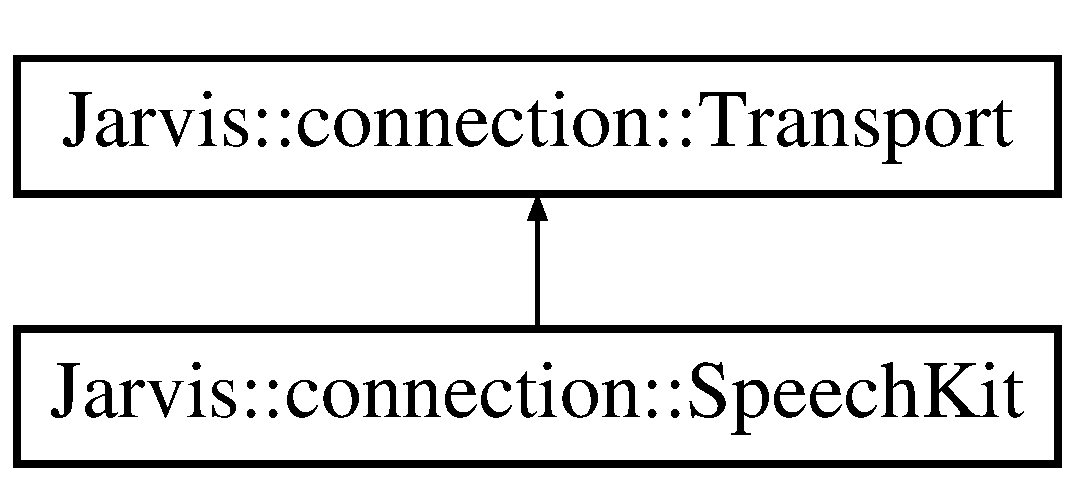
\includegraphics[height=2.000000cm]{classJarvis_1_1connection_1_1SpeechKit}
\end{center}
\end{figure}
\subsection*{Открытые члены}
\begin{DoxyCompactItemize}
\item 
\hyperlink{classJarvis_1_1connection_1_1SpeechKit_a814a5553551a585b66a7e72c99b3522f}{Speech\+Kit} (const Transport\+::j\+Path \&path, const Transport\+::\+Options\+List\+::yandex\+Options yandex\+Options)
\begin{DoxyCompactList}\small\item\em Конструктор \end{DoxyCompactList}\item 
\mbox{\Hypertarget{classJarvis_1_1connection_1_1SpeechKit_ae84ee36952ac6a4f2dfb9285d08ab4f6}\label{classJarvis_1_1connection_1_1SpeechKit_ae84ee36952ac6a4f2dfb9285d08ab4f6}} 
\hyperlink{classJarvis_1_1connection_1_1SpeechKit_ae84ee36952ac6a4f2dfb9285d08ab4f6}{$\sim$\+Speech\+Kit} ()=default
\begin{DoxyCompactList}\small\item\em Деструктор \end{DoxyCompactList}\item 
bool \hyperlink{classJarvis_1_1connection_1_1SpeechKit_af213e0c8c3f6bb8a1776f6f21c859713}{send} () override
\begin{DoxyCompactList}\small\item\em Отправка данных \end{DoxyCompactList}\item 
\mbox{\Hypertarget{classJarvis_1_1connection_1_1SpeechKit_a84d5ffcc555d07c4360bdbfaf3eb67c1}\label{classJarvis_1_1connection_1_1SpeechKit_a84d5ffcc555d07c4360bdbfaf3eb67c1}} 
void \hyperlink{classJarvis_1_1connection_1_1SpeechKit_a84d5ffcc555d07c4360bdbfaf3eb67c1}{set\+Options} () override
\begin{DoxyCompactList}\small\item\em Задание параметров отправки \end{DoxyCompactList}\item 
\mbox{\Hypertarget{classJarvis_1_1connection_1_1SpeechKit_a198b1b71454117a14939aa714e1a7d3e}\label{classJarvis_1_1connection_1_1SpeechKit_a198b1b71454117a14939aa714e1a7d3e}} 
{\bfseries Speech\+Kit} (const \hyperlink{classJarvis_1_1connection_1_1SpeechKit}{Speech\+Kit} \&copy)=delete
\item 
\mbox{\Hypertarget{classJarvis_1_1connection_1_1SpeechKit_ad9e08c9e8cc41e40c60f61f26c7b69d6}\label{classJarvis_1_1connection_1_1SpeechKit_ad9e08c9e8cc41e40c60f61f26c7b69d6}} 
\hyperlink{classJarvis_1_1connection_1_1SpeechKit}{Speech\+Kit} \& {\bfseries operator=} (const \hyperlink{classJarvis_1_1connection_1_1SpeechKit}{Speech\+Kit} \&copy)=delete
\end{DoxyCompactItemize}
\subsection*{Дополнительные унаследованные члены}


\subsection{Подробное описание}
Класс для \char`\"{}общения\char`\"{} с сервером Yandex\+Speech\+Kit\+Cloud. 

\subsection{Конструктор(ы)}
\mbox{\Hypertarget{classJarvis_1_1connection_1_1SpeechKit_a814a5553551a585b66a7e72c99b3522f}\label{classJarvis_1_1connection_1_1SpeechKit_a814a5553551a585b66a7e72c99b3522f}} 
\index{Jarvis\+::connection\+::\+Speech\+Kit@{Jarvis\+::connection\+::\+Speech\+Kit}!Speech\+Kit@{Speech\+Kit}}
\index{Speech\+Kit@{Speech\+Kit}!Jarvis\+::connection\+::\+Speech\+Kit@{Jarvis\+::connection\+::\+Speech\+Kit}}
\subsubsection{\texorpdfstring{Speech\+Kit()}{SpeechKit()}}
{\footnotesize\ttfamily Jarvis\+::connection\+::\+Speech\+Kit\+::\+Speech\+Kit (\begin{DoxyParamCaption}\item[{const Transport\+::j\+Path \&}]{path,  }\item[{const Transport\+::\+Options\+List\+::yandex\+Options}]{yandex\+Options }\end{DoxyParamCaption})}



Конструктор 


\begin{DoxyParams}{Аргументы}
{\em path} & Путь до конфигурационного файла \\
\hline
{\em yandex\+Options} & Список нужных ключей для конфигурационного файла \\
\hline
\end{DoxyParams}


\subsection{Методы}
\mbox{\Hypertarget{classJarvis_1_1connection_1_1SpeechKit_af213e0c8c3f6bb8a1776f6f21c859713}\label{classJarvis_1_1connection_1_1SpeechKit_af213e0c8c3f6bb8a1776f6f21c859713}} 
\index{Jarvis\+::connection\+::\+Speech\+Kit@{Jarvis\+::connection\+::\+Speech\+Kit}!send@{send}}
\index{send@{send}!Jarvis\+::connection\+::\+Speech\+Kit@{Jarvis\+::connection\+::\+Speech\+Kit}}
\subsubsection{\texorpdfstring{send()}{send()}}
{\footnotesize\ttfamily bool Jarvis\+::connection\+::\+Speech\+Kit\+::send (\begin{DoxyParamCaption}{ }\end{DoxyParamCaption})\hspace{0.3cm}{\ttfamily [override]}, {\ttfamily [virtual]}}



Отправка данных 

\begin{DoxyReturn}{Возвращает}
bool Подтверждение отправки 
\end{DoxyReturn}


Замещает \hyperlink{classJarvis_1_1connection_1_1Transport_ad0116f6773802fd75ea6795313051a96}{Jarvis\+::connection\+::\+Transport}.



Объявления и описания членов класса находятся в файле\+:\begin{DoxyCompactItemize}
\item 
/\+Users/vladislavpereskokov/\+Desktop/\+Jarvis/\+Voice/include/Speech\+Kit.\+hpp\end{DoxyCompactItemize}

\hypertarget{classJarvis_1_1connection_1_1Transport}{}\section{Класс Jarvis\+:\+:connection\+:\+:Transport}
\label{classJarvis_1_1connection_1_1Transport}\index{Jarvis\+::connection\+::\+Transport@{Jarvis\+::connection\+::\+Transport}}


Абстрактный класс для \char`\"{}общения\char`\"{} с сервером  




{\ttfamily \#include $<$Transport.\+hpp$>$}

Граф наследования\+:Jarvis\+:\+:connection\+:\+:Transport\+:\begin{figure}[H]
\begin{center}
\leavevmode
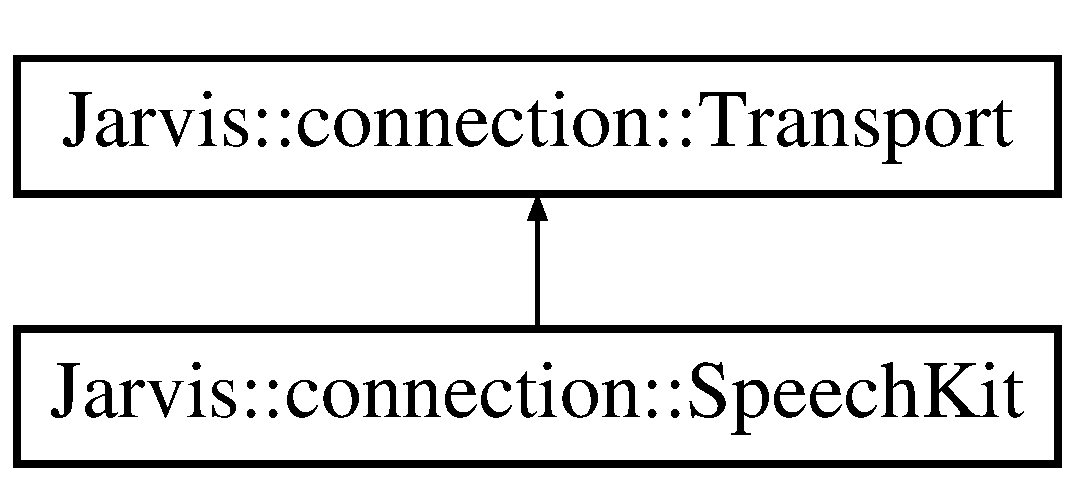
\includegraphics[height=2.000000cm]{classJarvis_1_1connection_1_1Transport}
\end{center}
\end{figure}
\subsection*{Открытые типы}
\begin{DoxyCompactItemize}
\item 
using \hyperlink{classJarvis_1_1connection_1_1Transport_a81b1e5dc6c0a246fa2a225a1ff185b95}{property} = \hyperlink{classJarvis_1_1connection_1_1Transport_a2cb5e9e28fa84404e8b002c65fe8ecd0}{Options\+List}
\begin{DoxyCompactList}\small\item\em Определяет тип для параметров отправки \end{DoxyCompactList}\end{DoxyCompactItemize}
\subsection*{Открытые члены}
\begin{DoxyCompactItemize}
\item 
\hyperlink{classJarvis_1_1connection_1_1Transport_a2cb5e9e28fa84404e8b002c65fe8ecd0}{Options\+List} (const j\+Path \&path, const yandex\+Options yandex\+Options)
\begin{DoxyCompactList}\small\item\em Конструктор \end{DoxyCompactList}\item 
option\+Value \hyperlink{classJarvis_1_1connection_1_1Transport_a46481607af9201bd96cd37f44ab3f02a}{get\+Option} (const option \&option)
\begin{DoxyCompactList}\small\item\em Метод получения значения параметра \end{DoxyCompactList}\item 
\mbox{\Hypertarget{classJarvis_1_1connection_1_1Transport_a6e9599cad725bc1d305908a0c6325511}\label{classJarvis_1_1connection_1_1Transport_a6e9599cad725bc1d305908a0c6325511}} 
\hyperlink{classJarvis_1_1connection_1_1Transport_a6e9599cad725bc1d305908a0c6325511}{$\sim$\+Options\+List} ()=default
\begin{DoxyCompactList}\small\item\em Деструктор \end{DoxyCompactList}\item 
\mbox{\Hypertarget{classJarvis_1_1connection_1_1Transport_ab80ef9d2e0ff34de3a81fe653fd66563}\label{classJarvis_1_1connection_1_1Transport_ab80ef9d2e0ff34de3a81fe653fd66563}} 
{\bfseries Options\+List} ()=delete
\item 
\mbox{\Hypertarget{classJarvis_1_1connection_1_1Transport_a8e67b3b2abea1422f25bf1fa583c3081}\label{classJarvis_1_1connection_1_1Transport_a8e67b3b2abea1422f25bf1fa583c3081}} 
{\bfseries Options\+List} (const Options\+List \&copy)=delete
\item 
\mbox{\Hypertarget{classJarvis_1_1connection_1_1Transport_ad32df85374b4ebe723e829521fde41ec}\label{classJarvis_1_1connection_1_1Transport_ad32df85374b4ebe723e829521fde41ec}} 
\hyperlink{classJarvis_1_1connection_1_1Transport_a2cb5e9e28fa84404e8b002c65fe8ecd0}{Options\+List} \& {\bfseries operator=} (const \hyperlink{classJarvis_1_1connection_1_1Transport_a2cb5e9e28fa84404e8b002c65fe8ecd0}{Options\+List} \&copy)=delete
\item 
void \hyperlink{classJarvis_1_1connection_1_1Transport_aeb9700e28a25af20c96beccf4b6b3aef}{fill\+List} (const j\+List \&list)
\begin{DoxyCompactList}\small\item\em Метод заполнения списка параметров \end{DoxyCompactList}\item 
url \hyperlink{classJarvis_1_1connection_1_1Transport_ab08175e845055cdd1ccbe7994f0c1973}{make\+Url} (const j\+List \&list, url \&url)
\begin{DoxyCompactList}\small\item\em Метод составления U\+RL\textquotesingle{}а из ключей и их значений для post запроса \end{DoxyCompactList}\item 
bool \hyperlink{classJarvis_1_1connection_1_1Transport_a41a2e836f9c20e4d4aae16ebcc895b8c}{find\+Yandex\+Option} (const yandex\+Option \&option)
\begin{DoxyCompactList}\small\item\em Метод поиска ключевых параметров \end{DoxyCompactList}\item 
\hyperlink{classJarvis_1_1connection_1_1Transport_a2fce583b7c16902b5c2f4ad492371e2c}{Transport} (const j\+Path \&path, const Options\+List\+::yandex\+Options yandex\+Options)
\begin{DoxyCompactList}\small\item\em Конструктор \end{DoxyCompactList}\item 
\mbox{\Hypertarget{classJarvis_1_1connection_1_1Transport_aa074aa7a32a3bf78ec64aba07984b502}\label{classJarvis_1_1connection_1_1Transport_aa074aa7a32a3bf78ec64aba07984b502}} 
virtual \hyperlink{classJarvis_1_1connection_1_1Transport_aa074aa7a32a3bf78ec64aba07984b502}{$\sim$\+Transport} ()
\begin{DoxyCompactList}\small\item\em Деструктор \end{DoxyCompactList}\item 
virtual bool \hyperlink{classJarvis_1_1connection_1_1Transport_ad0116f6773802fd75ea6795313051a96}{send} ()=0
\begin{DoxyCompactList}\small\item\em Отправка данных \end{DoxyCompactList}\item 
response\+String \hyperlink{classJarvis_1_1connection_1_1Transport_a25b1e13d35fe44466a4f5bdddd8ea499}{recv} () const
\begin{DoxyCompactList}\small\item\em Получение данных \end{DoxyCompactList}\item 
bool \hyperlink{classJarvis_1_1connection_1_1Transport_abce3b6342c4a90603b187485422828c6}{connect} ()
\begin{DoxyCompactList}\small\item\em Соединение \end{DoxyCompactList}\item 
bool \hyperlink{classJarvis_1_1connection_1_1Transport_a9b15d1e6a7be779dcf8284ff0f17a8b0}{is\+Connect} () const
\begin{DoxyCompactList}\small\item\em Проверка соединения \end{DoxyCompactList}\item 
bool \hyperlink{classJarvis_1_1connection_1_1Transport_ae97760ea03453e9621027051c99a1c72}{check\+Connection} (const socket $\ast$curl) const
\begin{DoxyCompactList}\small\item\em Проверка соединения \end{DoxyCompactList}\item 
\mbox{\Hypertarget{classJarvis_1_1connection_1_1Transport_aea38743d9d867274991c19f1747e6f11}\label{classJarvis_1_1connection_1_1Transport_aea38743d9d867274991c19f1747e6f11}} 
virtual void \hyperlink{classJarvis_1_1connection_1_1Transport_aea38743d9d867274991c19f1747e6f11}{set\+Options} ()=0
\begin{DoxyCompactList}\small\item\em Задание параметров отправки \end{DoxyCompactList}\item 
\mbox{\Hypertarget{classJarvis_1_1connection_1_1Transport_ab65f3a824a24bd7d33fb8bf8b191d3ca}\label{classJarvis_1_1connection_1_1Transport_ab65f3a824a24bd7d33fb8bf8b191d3ca}} 
{\bfseries Transport} (const \hyperlink{classJarvis_1_1connection_1_1Transport}{Transport} \&copy)=delete
\item 
\mbox{\Hypertarget{classJarvis_1_1connection_1_1Transport_ae8dc60fe1e4b9cdd7730674ced147000}\label{classJarvis_1_1connection_1_1Transport_ae8dc60fe1e4b9cdd7730674ced147000}} 
\hyperlink{classJarvis_1_1connection_1_1Transport}{Transport} \& {\bfseries operator=} (const \hyperlink{classJarvis_1_1connection_1_1Transport}{Transport} \&copy)=delete
\end{DoxyCompactItemize}
\subsection*{Открытые атрибуты}
\begin{DoxyCompactItemize}
\item 
protected \hyperlink{classJarvis_1_1connection_1_1Transport_ab70d89176c8abee3eb780fab5ab5dc63}{params}\+: option\+List \+\_\+opt\+List
\item 
private \hyperlink{classJarvis_1_1connection_1_1Transport_ad7b0a1aeb169584cbdc046b3ac613819}{params}\+: yandex\+Options \+\_\+yandex\+Options
\item 
\hyperlink{classJarvis_1_1connection_1_1Transport_a81b1e5dc6c0a246fa2a225a1ff185b95}{property} \hyperlink{classJarvis_1_1connection_1_1Transport_aff80004ef5bbfa118bc9388c04124df2}{\+\_\+properties}
\item 
header\+List $\ast$ \hyperlink{classJarvis_1_1connection_1_1Transport_aa28ff148972b44b6dc6a1523d674e9d3}{\+\_\+headers}
\item 
response \hyperlink{classJarvis_1_1connection_1_1Transport_afb6094003e40fda2f269d68b5ecdc7d2}{\+\_\+response}
\end{DoxyCompactItemize}


\subsection{Подробное описание}
Абстрактный класс для \char`\"{}общения\char`\"{} с сервером 

\subsection{Определения типов}
\mbox{\Hypertarget{classJarvis_1_1connection_1_1Transport_a81b1e5dc6c0a246fa2a225a1ff185b95}\label{classJarvis_1_1connection_1_1Transport_a81b1e5dc6c0a246fa2a225a1ff185b95}} 
\index{Jarvis\+::connection\+::\+Transport@{Jarvis\+::connection\+::\+Transport}!property@{property}}
\index{property@{property}!Jarvis\+::connection\+::\+Transport@{Jarvis\+::connection\+::\+Transport}}
\subsubsection{\texorpdfstring{property}{property}}
{\footnotesize\ttfamily using Jarvis\+::connection\+::\+Transport\+::property =  \hyperlink{classJarvis_1_1connection_1_1Transport_a2cb5e9e28fa84404e8b002c65fe8ecd0}{Options\+List}}



Определяет тип для параметров отправки 

Options\+List property 

\subsection{Конструктор(ы)}
\mbox{\Hypertarget{classJarvis_1_1connection_1_1Transport_a2fce583b7c16902b5c2f4ad492371e2c}\label{classJarvis_1_1connection_1_1Transport_a2fce583b7c16902b5c2f4ad492371e2c}} 
\index{Jarvis\+::connection\+::\+Transport@{Jarvis\+::connection\+::\+Transport}!Transport@{Transport}}
\index{Transport@{Transport}!Jarvis\+::connection\+::\+Transport@{Jarvis\+::connection\+::\+Transport}}
\subsubsection{\texorpdfstring{Transport()}{Transport()}}
{\footnotesize\ttfamily Jarvis\+::connection\+::\+Transport\+::\+Transport (\begin{DoxyParamCaption}\item[{const j\+Path \&}]{path,  }\item[{const Options\+List\+::yandex\+Options}]{yandex\+Options }\end{DoxyParamCaption})\hspace{0.3cm}{\ttfamily [explicit]}}



Конструктор 


\begin{DoxyParams}{Аргументы}
{\em path} & Путь до конфигурационного файла \\
\hline
{\em yandex\+Options} & Список нужных ключей для конфигурационного файла \\
\hline
\end{DoxyParams}


\subsection{Методы}
\mbox{\Hypertarget{classJarvis_1_1connection_1_1Transport_ae97760ea03453e9621027051c99a1c72}\label{classJarvis_1_1connection_1_1Transport_ae97760ea03453e9621027051c99a1c72}} 
\index{Jarvis\+::connection\+::\+Transport@{Jarvis\+::connection\+::\+Transport}!check\+Connection@{check\+Connection}}
\index{check\+Connection@{check\+Connection}!Jarvis\+::connection\+::\+Transport@{Jarvis\+::connection\+::\+Transport}}
\subsubsection{\texorpdfstring{check\+Connection()}{checkConnection()}}
{\footnotesize\ttfamily bool Jarvis\+::connection\+::\+Transport\+::check\+Connection (\begin{DoxyParamCaption}\item[{const socket $\ast$}]{curl }\end{DoxyParamCaption}) const}



Проверка соединения 


\begin{DoxyParams}{Аргументы}
{\em curl} & Сокет для проверки \\
\hline
\end{DoxyParams}
\begin{DoxyReturn}{Возвращает}
bool Подтверждение соединения 
\end{DoxyReturn}
\mbox{\Hypertarget{classJarvis_1_1connection_1_1Transport_abce3b6342c4a90603b187485422828c6}\label{classJarvis_1_1connection_1_1Transport_abce3b6342c4a90603b187485422828c6}} 
\index{Jarvis\+::connection\+::\+Transport@{Jarvis\+::connection\+::\+Transport}!connect@{connect}}
\index{connect@{connect}!Jarvis\+::connection\+::\+Transport@{Jarvis\+::connection\+::\+Transport}}
\subsubsection{\texorpdfstring{connect()}{connect()}}
{\footnotesize\ttfamily bool Jarvis\+::connection\+::\+Transport\+::connect (\begin{DoxyParamCaption}{ }\end{DoxyParamCaption})}



Соединение 

\begin{DoxyReturn}{Возвращает}
bool Подтверждение соединения 
\end{DoxyReturn}
\mbox{\Hypertarget{classJarvis_1_1connection_1_1Transport_aeb9700e28a25af20c96beccf4b6b3aef}\label{classJarvis_1_1connection_1_1Transport_aeb9700e28a25af20c96beccf4b6b3aef}} 
\index{Jarvis\+::connection\+::\+Transport@{Jarvis\+::connection\+::\+Transport}!fill\+List@{fill\+List}}
\index{fill\+List@{fill\+List}!Jarvis\+::connection\+::\+Transport@{Jarvis\+::connection\+::\+Transport}}
\subsubsection{\texorpdfstring{fill\+List()}{fillList()}}
{\footnotesize\ttfamily void Jarvis\+::connection\+::\+Transport\+::fill\+List (\begin{DoxyParamCaption}\item[{const j\+List \&}]{list }\end{DoxyParamCaption})}



Метод заполнения списка параметров 


\begin{DoxyParams}{Аргументы}
{\em list} & Отображение из распарсенного дерева \\
\hline
\end{DoxyParams}
\mbox{\Hypertarget{classJarvis_1_1connection_1_1Transport_a41a2e836f9c20e4d4aae16ebcc895b8c}\label{classJarvis_1_1connection_1_1Transport_a41a2e836f9c20e4d4aae16ebcc895b8c}} 
\index{Jarvis\+::connection\+::\+Transport@{Jarvis\+::connection\+::\+Transport}!find\+Yandex\+Option@{find\+Yandex\+Option}}
\index{find\+Yandex\+Option@{find\+Yandex\+Option}!Jarvis\+::connection\+::\+Transport@{Jarvis\+::connection\+::\+Transport}}
\subsubsection{\texorpdfstring{find\+Yandex\+Option()}{findYandexOption()}}
{\footnotesize\ttfamily bool Jarvis\+::connection\+::\+Transport\+::find\+Yandex\+Option (\begin{DoxyParamCaption}\item[{const yandex\+Option \&}]{option }\end{DoxyParamCaption})}



Метод поиска ключевых параметров 


\begin{DoxyParams}{Аргументы}
{\em option} & Искомый параметр \\
\hline
\end{DoxyParams}
\begin{DoxyReturn}{Возвращает}
bool Подтверждение -\/ найдено ли 
\end{DoxyReturn}
\mbox{\Hypertarget{classJarvis_1_1connection_1_1Transport_a46481607af9201bd96cd37f44ab3f02a}\label{classJarvis_1_1connection_1_1Transport_a46481607af9201bd96cd37f44ab3f02a}} 
\index{Jarvis\+::connection\+::\+Transport@{Jarvis\+::connection\+::\+Transport}!get\+Option@{get\+Option}}
\index{get\+Option@{get\+Option}!Jarvis\+::connection\+::\+Transport@{Jarvis\+::connection\+::\+Transport}}
\subsubsection{\texorpdfstring{get\+Option()}{getOption()}}
{\footnotesize\ttfamily option\+Value Jarvis\+::connection\+::\+Transport\+::get\+Option (\begin{DoxyParamCaption}\item[{const option \&}]{option }\end{DoxyParamCaption})}



Метод получения значения параметра 


\begin{DoxyParams}{Аргументы}
{\em option} & Искомый параметр \\
\hline
\end{DoxyParams}
\begin{DoxyReturn}{Возвращает}
option\+Value Значение заданного параметра 
\end{DoxyReturn}
\mbox{\Hypertarget{classJarvis_1_1connection_1_1Transport_a9b15d1e6a7be779dcf8284ff0f17a8b0}\label{classJarvis_1_1connection_1_1Transport_a9b15d1e6a7be779dcf8284ff0f17a8b0}} 
\index{Jarvis\+::connection\+::\+Transport@{Jarvis\+::connection\+::\+Transport}!is\+Connect@{is\+Connect}}
\index{is\+Connect@{is\+Connect}!Jarvis\+::connection\+::\+Transport@{Jarvis\+::connection\+::\+Transport}}
\subsubsection{\texorpdfstring{is\+Connect()}{isConnect()}}
{\footnotesize\ttfamily bool Jarvis\+::connection\+::\+Transport\+::is\+Connect (\begin{DoxyParamCaption}{ }\end{DoxyParamCaption}) const}



Проверка соединения 

\begin{DoxyReturn}{Возвращает}
bool Подтверждение соединения 
\end{DoxyReturn}
\mbox{\Hypertarget{classJarvis_1_1connection_1_1Transport_ab08175e845055cdd1ccbe7994f0c1973}\label{classJarvis_1_1connection_1_1Transport_ab08175e845055cdd1ccbe7994f0c1973}} 
\index{Jarvis\+::connection\+::\+Transport@{Jarvis\+::connection\+::\+Transport}!make\+Url@{make\+Url}}
\index{make\+Url@{make\+Url}!Jarvis\+::connection\+::\+Transport@{Jarvis\+::connection\+::\+Transport}}
\subsubsection{\texorpdfstring{make\+Url()}{makeUrl()}}
{\footnotesize\ttfamily url Jarvis\+::connection\+::\+Transport\+::make\+Url (\begin{DoxyParamCaption}\item[{const j\+List \&}]{list,  }\item[{url \&}]{url }\end{DoxyParamCaption})}



Метод составления U\+RL\textquotesingle{}а из ключей и их значений для post запроса 


\begin{DoxyParams}{Аргументы}
{\em list} & Отображение из распарсенного дерева \\
\hline
{\em url} & Сырой url \\
\hline
\end{DoxyParams}
\begin{DoxyReturn}{Возвращает}
url U\+RL для отправки 
\end{DoxyReturn}
\mbox{\Hypertarget{classJarvis_1_1connection_1_1Transport_a2cb5e9e28fa84404e8b002c65fe8ecd0}\label{classJarvis_1_1connection_1_1Transport_a2cb5e9e28fa84404e8b002c65fe8ecd0}} 
\index{Jarvis\+::connection\+::\+Transport@{Jarvis\+::connection\+::\+Transport}!Options\+List@{Options\+List}}
\index{Options\+List@{Options\+List}!Jarvis\+::connection\+::\+Transport@{Jarvis\+::connection\+::\+Transport}}
\subsubsection{\texorpdfstring{Options\+List()}{OptionsList()}}
{\footnotesize\ttfamily Jarvis\+::connection\+::\+Transport\+::\+Options\+List (\begin{DoxyParamCaption}\item[{const j\+Path \&}]{path,  }\item[{const yandex\+Options}]{yandex\+Options }\end{DoxyParamCaption})\hspace{0.3cm}{\ttfamily [explicit]}}



Конструктор 


\begin{DoxyParams}{Аргументы}
{\em path} & Путь до конфигурационного файла \\
\hline
{\em yandex\+Options} & Список с необходимыми ключами \\
\hline
\end{DoxyParams}
\mbox{\Hypertarget{classJarvis_1_1connection_1_1Transport_a25b1e13d35fe44466a4f5bdddd8ea499}\label{classJarvis_1_1connection_1_1Transport_a25b1e13d35fe44466a4f5bdddd8ea499}} 
\index{Jarvis\+::connection\+::\+Transport@{Jarvis\+::connection\+::\+Transport}!recv@{recv}}
\index{recv@{recv}!Jarvis\+::connection\+::\+Transport@{Jarvis\+::connection\+::\+Transport}}
\subsubsection{\texorpdfstring{recv()}{recv()}}
{\footnotesize\ttfamily response\+String Jarvis\+::connection\+::\+Transport\+::recv (\begin{DoxyParamCaption}{ }\end{DoxyParamCaption}) const}



Получение данных 

\begin{DoxyReturn}{Возвращает}
response\+String Полученное сообщение 
\end{DoxyReturn}
\mbox{\Hypertarget{classJarvis_1_1connection_1_1Transport_ad0116f6773802fd75ea6795313051a96}\label{classJarvis_1_1connection_1_1Transport_ad0116f6773802fd75ea6795313051a96}} 
\index{Jarvis\+::connection\+::\+Transport@{Jarvis\+::connection\+::\+Transport}!send@{send}}
\index{send@{send}!Jarvis\+::connection\+::\+Transport@{Jarvis\+::connection\+::\+Transport}}
\subsubsection{\texorpdfstring{send()}{send()}}
{\footnotesize\ttfamily virtual bool Jarvis\+::connection\+::\+Transport\+::send (\begin{DoxyParamCaption}{ }\end{DoxyParamCaption})\hspace{0.3cm}{\ttfamily [pure virtual]}}



Отправка данных 

\begin{DoxyReturn}{Возвращает}
bool Подтверждение отправки 
\end{DoxyReturn}


Замещается в \hyperlink{classJarvis_1_1connection_1_1SpeechKit_af213e0c8c3f6bb8a1776f6f21c859713}{Jarvis\+::connection\+::\+Speech\+Kit}.



\subsection{Данные класса}
\mbox{\Hypertarget{classJarvis_1_1connection_1_1Transport_aa28ff148972b44b6dc6a1523d674e9d3}\label{classJarvis_1_1connection_1_1Transport_aa28ff148972b44b6dc6a1523d674e9d3}} 
\index{Jarvis\+::connection\+::\+Transport@{Jarvis\+::connection\+::\+Transport}!\+\_\+headers@{\+\_\+headers}}
\index{\+\_\+headers@{\+\_\+headers}!Jarvis\+::connection\+::\+Transport@{Jarvis\+::connection\+::\+Transport}}
\subsubsection{\texorpdfstring{\+\_\+headers}{\_headers}}
{\footnotesize\ttfamily header\+List$\ast$ Jarvis\+::connection\+::\+Transport\+::\+\_\+headers}

Заголовки \mbox{\Hypertarget{classJarvis_1_1connection_1_1Transport_aff80004ef5bbfa118bc9388c04124df2}\label{classJarvis_1_1connection_1_1Transport_aff80004ef5bbfa118bc9388c04124df2}} 
\index{Jarvis\+::connection\+::\+Transport@{Jarvis\+::connection\+::\+Transport}!\+\_\+properties@{\+\_\+properties}}
\index{\+\_\+properties@{\+\_\+properties}!Jarvis\+::connection\+::\+Transport@{Jarvis\+::connection\+::\+Transport}}
\subsubsection{\texorpdfstring{\+\_\+properties}{\_properties}}
{\footnotesize\ttfamily \hyperlink{classJarvis_1_1connection_1_1Transport_a81b1e5dc6c0a246fa2a225a1ff185b95}{property} Jarvis\+::connection\+::\+Transport\+::\+\_\+properties}

Параметры соединения \mbox{\Hypertarget{classJarvis_1_1connection_1_1Transport_afb6094003e40fda2f269d68b5ecdc7d2}\label{classJarvis_1_1connection_1_1Transport_afb6094003e40fda2f269d68b5ecdc7d2}} 
\index{Jarvis\+::connection\+::\+Transport@{Jarvis\+::connection\+::\+Transport}!\+\_\+response@{\+\_\+response}}
\index{\+\_\+response@{\+\_\+response}!Jarvis\+::connection\+::\+Transport@{Jarvis\+::connection\+::\+Transport}}
\subsubsection{\texorpdfstring{\+\_\+response}{\_response}}
{\footnotesize\ttfamily response Jarvis\+::connection\+::\+Transport\+::\+\_\+response}

Ответ с сервера \mbox{\Hypertarget{classJarvis_1_1connection_1_1Transport_ab70d89176c8abee3eb780fab5ab5dc63}\label{classJarvis_1_1connection_1_1Transport_ab70d89176c8abee3eb780fab5ab5dc63}} 
\index{Jarvis\+::connection\+::\+Transport@{Jarvis\+::connection\+::\+Transport}!params@{params}}
\index{params@{params}!Jarvis\+::connection\+::\+Transport@{Jarvis\+::connection\+::\+Transport}}
\subsubsection{\texorpdfstring{params}{params}\hspace{0.1cm}{\footnotesize\ttfamily [1/2]}}
{\footnotesize\ttfamily protected Jarvis\+::connection\+::\+Transport\+::params}

Список параметров

Сокет \mbox{\Hypertarget{classJarvis_1_1connection_1_1Transport_ad7b0a1aeb169584cbdc046b3ac613819}\label{classJarvis_1_1connection_1_1Transport_ad7b0a1aeb169584cbdc046b3ac613819}} 
\index{Jarvis\+::connection\+::\+Transport@{Jarvis\+::connection\+::\+Transport}!params@{params}}
\index{params@{params}!Jarvis\+::connection\+::\+Transport@{Jarvis\+::connection\+::\+Transport}}
\subsubsection{\texorpdfstring{params}{params}\hspace{0.1cm}{\footnotesize\ttfamily [2/2]}}
{\footnotesize\ttfamily private Jarvis\+::connection\+::\+Transport\+::params}

Список ключевых параметров 

Объявления и описания членов класса находятся в файле\+:\begin{DoxyCompactItemize}
\item 
/\+Users/vladislavpereskokov/\+Desktop/\+Jarvis/\+Voice/include/Transport.\+hpp\end{DoxyCompactItemize}

\hypertarget{classJarvis_1_1Voice}{}\section{Класс Jarvis\+:\+:Voice}
\label{classJarvis_1_1Voice}\index{Jarvis\+::\+Voice@{Jarvis\+::\+Voice}}


Описывает объект голос  




{\ttfamily \#include $<$Voice.\+hpp$>$}

\subsection*{Открытые члены}
\begin{DoxyCompactItemize}
\item 
\hyperlink{classJarvis_1_1Voice_a79c708aebcb92b2d3f74de9992f1082a}{Voice} (const path \&path, const name \&name)
\begin{DoxyCompactList}\small\item\em Конструктор \end{DoxyCompactList}\item 
\mbox{\Hypertarget{classJarvis_1_1Voice_a6bb0bc7ce0a275c03b8cc1b7cd45ea7e}\label{classJarvis_1_1Voice_a6bb0bc7ce0a275c03b8cc1b7cd45ea7e}} 
\hyperlink{classJarvis_1_1Voice_a6bb0bc7ce0a275c03b8cc1b7cd45ea7e}{$\sim$\+Voice} ()=default
\begin{DoxyCompactList}\small\item\em Деструктор \end{DoxyCompactList}\item 
\hyperlink{classJarvis_1_1Voice_ab1b0b2c2bb6d175b34970086cce05245}{Voice} (const \hyperlink{classJarvis_1_1Voice}{Voice} \&copy)=default
\begin{DoxyCompactList}\small\item\em Конструктор копирования \end{DoxyCompactList}\item 
\hyperlink{classJarvis_1_1Voice_a3bac269758c6f299fbd1c661f3154747}{Voice} (\hyperlink{classJarvis_1_1Voice}{Voice} \&\&copy)=default
\begin{DoxyCompactList}\small\item\em Конструктор копирования \end{DoxyCompactList}\item 
\hyperlink{classJarvis_1_1Voice}{Voice} \& \hyperlink{classJarvis_1_1Voice_ab90791a6daeab735274366ca8ce69da2}{operator=} (const \hyperlink{classJarvis_1_1Voice}{Voice} \&copy)=default
\begin{DoxyCompactList}\small\item\em Конструктор копирования \end{DoxyCompactList}\item 
\hyperlink{classJarvis_1_1Voice}{Voice} \& \hyperlink{classJarvis_1_1Voice_a16477e744cf7f448f10d5bf37644ed15}{operator=} (\hyperlink{classJarvis_1_1Voice}{Voice} \&\&copy)=default
\begin{DoxyCompactList}\small\item\em Конструктор копирования \end{DoxyCompactList}\item 
bool \hyperlink{classJarvis_1_1Voice_ab86096f38092a5e0decd804588fb334c}{say} ()
\begin{DoxyCompactList}\small\item\em Конструктор копирования \end{DoxyCompactList}\item 
void \hyperlink{classJarvis_1_1Voice_a3be7bee43cebb0e1ef50a24b399a6954}{set\+Sentence} (const \hyperlink{classJarvis_1_1Sentence}{Sentence} \&sentence)
\begin{DoxyCompactList}\small\item\em Метод изменения фразы \end{DoxyCompactList}\item 
\hyperlink{classJarvis_1_1Sentence}{Sentence} \hyperlink{classJarvis_1_1Voice_ad1f37700f0f76426d34ba31a342505e8}{get\+Sentence} () const
\begin{DoxyCompactList}\small\item\em Метод получения фразы \end{DoxyCompactList}\item 
bool \hyperlink{classJarvis_1_1Voice_aacc05388ae250c1e515f993159443dff}{execute} ()
\begin{DoxyCompactList}\small\item\em Метод запуска воспроизведения голоса \end{DoxyCompactList}\item 
bool \hyperlink{classJarvis_1_1Voice_a509a6161183e0f2f8053371e621379ea}{find\+Command} (const connection\+::\+Map \&waves, const \hyperlink{classJarvis_1_1Sentence}{Sentence} \&sentence)
\begin{DoxyCompactList}\small\item\em Метод нахождения нужной команды \end{DoxyCompactList}\end{DoxyCompactItemize}
\subsection*{Открытые атрибуты}
\begin{DoxyCompactItemize}
\item 
private \hyperlink{classJarvis_1_1Voice_a23e07f1f4dfbe872ff95b53e32bad443}{params}\+: name \+\_\+name
\item 
map \hyperlink{classJarvis_1_1Voice_a70bc48a33f97bd1cf3b43e08824a041c}{\+\_\+waves}
\item 
\hyperlink{classJarvis_1_1Sentence}{Sentence} \hyperlink{classJarvis_1_1Voice_ac0a2f9e53d5b74b3ad7e84b0f203d4c4}{\+\_\+sentence}
\end{DoxyCompactItemize}


\subsection{Подробное описание}
Описывает объект голос 

\subsection{Конструктор(ы)}
\mbox{\Hypertarget{classJarvis_1_1Voice_a79c708aebcb92b2d3f74de9992f1082a}\label{classJarvis_1_1Voice_a79c708aebcb92b2d3f74de9992f1082a}} 
\index{Jarvis\+::\+Voice@{Jarvis\+::\+Voice}!Voice@{Voice}}
\index{Voice@{Voice}!Jarvis\+::\+Voice@{Jarvis\+::\+Voice}}
\subsubsection{\texorpdfstring{Voice()}{Voice()}\hspace{0.1cm}{\footnotesize\ttfamily [1/3]}}
{\footnotesize\ttfamily Jarvis\+::\+Voice\+::\+Voice (\begin{DoxyParamCaption}\item[{const path \&}]{path,  }\item[{const name \&}]{name }\end{DoxyParamCaption})}



Конструктор 


\begin{DoxyParams}{Аргументы}
{\em path} & Путь до конфигурационного файла \\
\hline
{\em name} & Имя голоса \\
\hline
\end{DoxyParams}
\mbox{\Hypertarget{classJarvis_1_1Voice_ab1b0b2c2bb6d175b34970086cce05245}\label{classJarvis_1_1Voice_ab1b0b2c2bb6d175b34970086cce05245}} 
\index{Jarvis\+::\+Voice@{Jarvis\+::\+Voice}!Voice@{Voice}}
\index{Voice@{Voice}!Jarvis\+::\+Voice@{Jarvis\+::\+Voice}}
\subsubsection{\texorpdfstring{Voice()}{Voice()}\hspace{0.1cm}{\footnotesize\ttfamily [2/3]}}
{\footnotesize\ttfamily Jarvis\+::\+Voice\+::\+Voice (\begin{DoxyParamCaption}\item[{const \hyperlink{classJarvis_1_1Voice}{Voice} \&}]{copy }\end{DoxyParamCaption})\hspace{0.3cm}{\ttfamily [default]}}



Конструктор копирования 


\begin{DoxyParams}{Аргументы}
{\em copy} & Копируемый объект \\
\hline
\end{DoxyParams}
\mbox{\Hypertarget{classJarvis_1_1Voice_a3bac269758c6f299fbd1c661f3154747}\label{classJarvis_1_1Voice_a3bac269758c6f299fbd1c661f3154747}} 
\index{Jarvis\+::\+Voice@{Jarvis\+::\+Voice}!Voice@{Voice}}
\index{Voice@{Voice}!Jarvis\+::\+Voice@{Jarvis\+::\+Voice}}
\subsubsection{\texorpdfstring{Voice()}{Voice()}\hspace{0.1cm}{\footnotesize\ttfamily [3/3]}}
{\footnotesize\ttfamily Jarvis\+::\+Voice\+::\+Voice (\begin{DoxyParamCaption}\item[{\hyperlink{classJarvis_1_1Voice}{Voice} \&\&}]{copy }\end{DoxyParamCaption})\hspace{0.3cm}{\ttfamily [default]}}



Конструктор копирования 


\begin{DoxyParams}{Аргументы}
{\em copy} & Копируемый объект \\
\hline
\end{DoxyParams}


\subsection{Методы}
\mbox{\Hypertarget{classJarvis_1_1Voice_aacc05388ae250c1e515f993159443dff}\label{classJarvis_1_1Voice_aacc05388ae250c1e515f993159443dff}} 
\index{Jarvis\+::\+Voice@{Jarvis\+::\+Voice}!execute@{execute}}
\index{execute@{execute}!Jarvis\+::\+Voice@{Jarvis\+::\+Voice}}
\subsubsection{\texorpdfstring{execute()}{execute()}}
{\footnotesize\ttfamily bool Jarvis\+::\+Voice\+::execute (\begin{DoxyParamCaption}{ }\end{DoxyParamCaption})}



Метод запуска воспроизведения голоса 

\begin{DoxyReturn}{Возвращает}
bool Проверка -\/ запустилось ли 
\end{DoxyReturn}
\mbox{\Hypertarget{classJarvis_1_1Voice_a509a6161183e0f2f8053371e621379ea}\label{classJarvis_1_1Voice_a509a6161183e0f2f8053371e621379ea}} 
\index{Jarvis\+::\+Voice@{Jarvis\+::\+Voice}!find\+Command@{find\+Command}}
\index{find\+Command@{find\+Command}!Jarvis\+::\+Voice@{Jarvis\+::\+Voice}}
\subsubsection{\texorpdfstring{find\+Command()}{findCommand()}}
{\footnotesize\ttfamily bool Jarvis\+::\+Voice\+::find\+Command (\begin{DoxyParamCaption}\item[{const connection\+::\+Map \&}]{waves,  }\item[{const \hyperlink{classJarvis_1_1Sentence}{Sentence} \&}]{sentence }\end{DoxyParamCaption})}



Метод нахождения нужной команды 


\begin{DoxyParams}{Аргументы}
{\em waves} & Сэмплы \\
\hline
{\em sentence} & Фраза \\
\hline
\end{DoxyParams}
\begin{DoxyReturn}{Возвращает}
bool Найдено ли 
\end{DoxyReturn}
\mbox{\Hypertarget{classJarvis_1_1Voice_ad1f37700f0f76426d34ba31a342505e8}\label{classJarvis_1_1Voice_ad1f37700f0f76426d34ba31a342505e8}} 
\index{Jarvis\+::\+Voice@{Jarvis\+::\+Voice}!get\+Sentence@{get\+Sentence}}
\index{get\+Sentence@{get\+Sentence}!Jarvis\+::\+Voice@{Jarvis\+::\+Voice}}
\subsubsection{\texorpdfstring{get\+Sentence()}{getSentence()}}
{\footnotesize\ttfamily \hyperlink{classJarvis_1_1Sentence}{Sentence} Jarvis\+::\+Voice\+::get\+Sentence (\begin{DoxyParamCaption}{ }\end{DoxyParamCaption}) const}



Метод получения фразы 

\begin{DoxyReturn}{Возвращает}
sentence Предложение 
\end{DoxyReturn}
\mbox{\Hypertarget{classJarvis_1_1Voice_ab90791a6daeab735274366ca8ce69da2}\label{classJarvis_1_1Voice_ab90791a6daeab735274366ca8ce69da2}} 
\index{Jarvis\+::\+Voice@{Jarvis\+::\+Voice}!operator=@{operator=}}
\index{operator=@{operator=}!Jarvis\+::\+Voice@{Jarvis\+::\+Voice}}
\subsubsection{\texorpdfstring{operator=()}{operator=()}\hspace{0.1cm}{\footnotesize\ttfamily [1/2]}}
{\footnotesize\ttfamily \hyperlink{classJarvis_1_1Voice}{Voice}\& Jarvis\+::\+Voice\+::operator= (\begin{DoxyParamCaption}\item[{const \hyperlink{classJarvis_1_1Voice}{Voice} \&}]{copy }\end{DoxyParamCaption})\hspace{0.3cm}{\ttfamily [default]}}



Конструктор копирования 


\begin{DoxyParams}{Аргументы}
{\em copy} & Копируемый объект \\
\hline
\end{DoxyParams}
\mbox{\Hypertarget{classJarvis_1_1Voice_a16477e744cf7f448f10d5bf37644ed15}\label{classJarvis_1_1Voice_a16477e744cf7f448f10d5bf37644ed15}} 
\index{Jarvis\+::\+Voice@{Jarvis\+::\+Voice}!operator=@{operator=}}
\index{operator=@{operator=}!Jarvis\+::\+Voice@{Jarvis\+::\+Voice}}
\subsubsection{\texorpdfstring{operator=()}{operator=()}\hspace{0.1cm}{\footnotesize\ttfamily [2/2]}}
{\footnotesize\ttfamily \hyperlink{classJarvis_1_1Voice}{Voice}\& Jarvis\+::\+Voice\+::operator= (\begin{DoxyParamCaption}\item[{\hyperlink{classJarvis_1_1Voice}{Voice} \&\&}]{copy }\end{DoxyParamCaption})\hspace{0.3cm}{\ttfamily [default]}}



Конструктор копирования 


\begin{DoxyParams}{Аргументы}
{\em copy} & Копируемый объект \\
\hline
\end{DoxyParams}
\mbox{\Hypertarget{classJarvis_1_1Voice_ab86096f38092a5e0decd804588fb334c}\label{classJarvis_1_1Voice_ab86096f38092a5e0decd804588fb334c}} 
\index{Jarvis\+::\+Voice@{Jarvis\+::\+Voice}!say@{say}}
\index{say@{say}!Jarvis\+::\+Voice@{Jarvis\+::\+Voice}}
\subsubsection{\texorpdfstring{say()}{say()}}
{\footnotesize\ttfamily bool Jarvis\+::\+Voice\+::say (\begin{DoxyParamCaption}{ }\end{DoxyParamCaption})}



Конструктор копирования 

\begin{DoxyReturn}{Возвращает}
bool Подтверждение -\/ была ли сказана фраза 
\end{DoxyReturn}
\mbox{\Hypertarget{classJarvis_1_1Voice_a3be7bee43cebb0e1ef50a24b399a6954}\label{classJarvis_1_1Voice_a3be7bee43cebb0e1ef50a24b399a6954}} 
\index{Jarvis\+::\+Voice@{Jarvis\+::\+Voice}!set\+Sentence@{set\+Sentence}}
\index{set\+Sentence@{set\+Sentence}!Jarvis\+::\+Voice@{Jarvis\+::\+Voice}}
\subsubsection{\texorpdfstring{set\+Sentence()}{setSentence()}}
{\footnotesize\ttfamily void Jarvis\+::\+Voice\+::set\+Sentence (\begin{DoxyParamCaption}\item[{const \hyperlink{classJarvis_1_1Sentence}{Sentence} \&}]{sentence }\end{DoxyParamCaption})}



Метод изменения фразы 


\begin{DoxyParams}{Аргументы}
{\em sentence} & Предложение \\
\hline
\end{DoxyParams}


\subsection{Данные класса}
\mbox{\Hypertarget{classJarvis_1_1Voice_ac0a2f9e53d5b74b3ad7e84b0f203d4c4}\label{classJarvis_1_1Voice_ac0a2f9e53d5b74b3ad7e84b0f203d4c4}} 
\index{Jarvis\+::\+Voice@{Jarvis\+::\+Voice}!\+\_\+sentence@{\+\_\+sentence}}
\index{\+\_\+sentence@{\+\_\+sentence}!Jarvis\+::\+Voice@{Jarvis\+::\+Voice}}
\subsubsection{\texorpdfstring{\+\_\+sentence}{\_sentence}}
{\footnotesize\ttfamily \hyperlink{classJarvis_1_1Sentence}{Sentence} Jarvis\+::\+Voice\+::\+\_\+sentence}

Фраза \mbox{\Hypertarget{classJarvis_1_1Voice_a70bc48a33f97bd1cf3b43e08824a041c}\label{classJarvis_1_1Voice_a70bc48a33f97bd1cf3b43e08824a041c}} 
\index{Jarvis\+::\+Voice@{Jarvis\+::\+Voice}!\+\_\+waves@{\+\_\+waves}}
\index{\+\_\+waves@{\+\_\+waves}!Jarvis\+::\+Voice@{Jarvis\+::\+Voice}}
\subsubsection{\texorpdfstring{\+\_\+waves}{\_waves}}
{\footnotesize\ttfamily map Jarvis\+::\+Voice\+::\+\_\+waves}

Необходимый сэмпл \mbox{\Hypertarget{classJarvis_1_1Voice_a23e07f1f4dfbe872ff95b53e32bad443}\label{classJarvis_1_1Voice_a23e07f1f4dfbe872ff95b53e32bad443}} 
\index{Jarvis\+::\+Voice@{Jarvis\+::\+Voice}!params@{params}}
\index{params@{params}!Jarvis\+::\+Voice@{Jarvis\+::\+Voice}}
\subsubsection{\texorpdfstring{params}{params}}
{\footnotesize\ttfamily private Jarvis\+::\+Voice\+::params}

Имя голоса 

Объявления и описания членов класса находятся в файле\+:\begin{DoxyCompactItemize}
\item 
/\+Users/vladislavpereskokov/\+Desktop/\+Jarvis/\+Voice/include/Voice.\+hpp\end{DoxyCompactItemize}

%--- End generated contents ---

% Index
\backmatter
\newpage
\phantomsection
\clearemptydoublepage
\addcontentsline{toc}{chapter}{Алфавитный указатель}
\printindex

\end{document}
